%
% Method
%

% !TEX root = ../../main.tex

\chapter{Methoden\label{sec:method}}

  \section{Design der Individuen}

    Der Ansatz für das Design der Individuen ist an \Glspl{Hexapod} angelehnt.
    Dabei sind viele Eigenschaften der Ameise in den Entwurf eingeflossen.
    Sie bieten mit ihren 6 Beinen eine gute Kombination aus Stabilität und Einfachheit der Steuerung.

    \subsection{Körper\label{sub:DesignBody}}

      Die Form des Körpers soll frei evolvierbar sein.
      Deshalb wird der Körper eines Individuums als Polygon mit \(n\) Punkten beschrieben.
      \\
      Als Einschränkung wird festgelegt, dass ein Polygon aus minimal 4 und maximal 8 Punkte generiert wird.
      Diese Bedingung beschränkt sowohl den Rechenaufwand der Berechnung des Körpers während der Simulation~(\vref{sec:simulation}),
      als auch in der Mutationsphase~(\vref{sec:Mutation}).
      Weiter wird festgelegt, dass das Polygon ein \gls{SimplePolygon} sein muss.
      Ohne diese Bedingung könnten Körper generiert werden, deren Kanten sich überkreuzen.
      Solche Körper werden als ungültig erachtet, da diese in der Natur nicht vorkommen.

      \begin{figure}[H]
        \centering
        \begin{subfigure}[b]{0.3\textwidth}
          %
% Concept body with 6 points
%

% !TEX root = ../main.tex

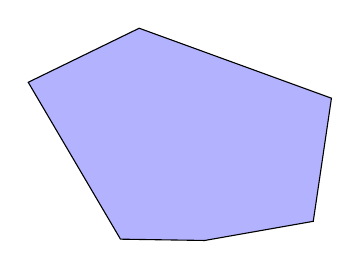
\begin{tikzpicture}[scale=\textwidth/3cm]

  \coordinate (P0) at (30:0.5cm);
  \coordinate (P1) at (110:0.5cm);
  \coordinate (P2) at (150:0.6cm);
  \coordinate (P3) at (220:0.3cm);
  \coordinate (P4) at (280:0.2cm);
  \coordinate (P5) at (340:0.4cm);

  % Draw lines between body points
  \draw [fill=blue, fill opacity=0.3] (P0) -- (P1) -- (P2) -- (P3) -- (P4) -- (P5) -- cycle;

\end{tikzpicture}

          \caption{6 Punkte\label{fig:ConceptBodyPoints6}}
        \end{subfigure}
        \qquad
        \begin{subfigure}[b]{0.3\textwidth}
          %
% Concept body with 8 points
%

% !TEX root = ../main.tex

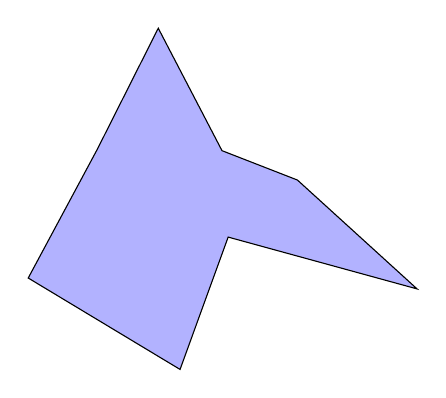
\begin{tikzpicture}[scale=\textwidth/3cm]

  \coordinate (P0) at (20:0.3cm);
  \coordinate (P1) at (77:0.2cm);
  \coordinate (P2) at (105:0.6cm);
  \coordinate (P3) at (150:0.4cm);
  \coordinate (P4) at (200:0.6cm);
  \coordinate (P5) at (260:0.5cm);
  \coordinate (P6) at (310:0.1cm);
  \coordinate (P7) at (340:0.7cm);

  % Draw lines between body points
  \draw [fill=blue, fill opacity=0.3] (P0) -- (P1) -- (P2) -- (P3) -- (P4) -- (P5) -- (P6) -- (P7) -- cycle;

\end{tikzpicture}

          \caption{8 Punkte\label{fig:ConceptBodyPoints8}}
        \end{subfigure}
        \caption{Konzept Körper\label{fig:ConceptBodyPoints}}
      \end{figure}

      \subsubsection{Hypothese zu Körperpunkten\label{subsub:hypoKp}}

        Es wird die Hypothese aufgestellt,
        dass sich ein Individuum mit 8 Körperpunkten schneller durch den Parcours bewegt,
        als ein Individuum mit weniger Körperpunkten.
        Die Vermutung dabei ist, dass durch die komplexere Form des Individuums die Balance besser gehalten werden kann.
        Im~\vref{chap:Resultate} und~\vref{chap:perspective} wird diskutiert, ob dies zutrifft.

    \subsection{Beine\label{sub:Beine}}

      Da als Grundkonzept ein \gls{Hexapod} verwendet wird, wird auch die Eigenschaft übernommen,
      dass das Individuum 6 Beine besitzt.
      Analog zu einer Ameise werden die Beine in 3 symmetrische Beinpaare aufgeteilt.
      \\
      Technisch bietet sich die Möglichkeit, die Beine nicht in Paare zu gliedern und asymmetrisch am Körper anzubringen.
      Doch in der Natur existiert eine solche Anordnung nicht, weshalb darauf verzichtet wird.
      \\
      \\
      Ein Bein ist unterteilt in Oberschenkel \(T\) und Unterschenkel \(S\).
      Die Höhe \(h_{l}\) und Breite \(w_{l}\) des Beins sind limitiert.
      Andernfalls ist anzunehmen, dass ungewünschte Resultate entstehen~\vref{sub:IntroReqLimit}.
      \\
      Im Genom bestimmt der Wert des Höhenfaktors \(h_{f}\),
      wie das Verhältnis der Länge von Unterschenkel \(h_{s}\) zu Oberschenkel \(h_{t}\) ist.
      \\
      Die Schenkel sind durch das Kniegelenk \(j_{k}\) miteinander verbunden.
      Mit dem Hüftgelenk \(j_{h}\) wird das Bein mit dem Körper verbunden.
      Für die Position des Hüftgelenkes existiert die Bedingung,
      dass das Gelenk innerhalb der Körperfläche angebracht sein muss.
      \\
      Zur Vereinfachung wird die Höhe jedes Gelenkes auf 0 festgelegt.

      \begin{figure}[H]
        \centering
        %
% Concept leg
%

% !TEX root = ../main.tex

\begin{tikzpicture}[scale=0.4]

  %def
  \tkzInit[xmin=-15,xmax=12,ymin=-6,ymax=12]
  \tkzDrawXY[noticks]
  \tkzDefPoints{-6/4/C1, 2/1/C2,0.205/6.548/A,-3/-2/B}

  %drawing
  \tkzDrawPoints(A,B)
  \tkzDrawSegments[gray](C1,C2)
  \tkzDrawSegments[red](C2,A C2,B)
  \tkzDrawSegments[blue](C1,A C1,B)
  \tkzDrawCircle(C1,A)
  \tkzDrawCircle(C2,A)
  % notation
  \tkzLabelPoints(C2)
  \tkzLabelPoints[left](C1)
  \tkzLabelPoints[above](A)
  \tkzLabelPoints[below](B)
  \tkzMarkSegment[color=blue,pos=.5,mark=||](C1,B)
  \tkzMarkSegment[color=red,pos=.5,mark=|](B,C2)
  \tkzMarkSegment[color=blue,pos=.5,mark=||](C1,A)
  \tkzMarkSegment[color=red,pos=.5,mark=|](A,C2)
  \tkzMarkRightAngle[size=0.7](C1,A,C2)
  \tkzMarkRightAngle[size=0.7](C1,B,C2)
  \tkzLabelCircle[above left](C1,A)(180){$K_1$}
  \tkzLabelCircle[right](C2,A)(-60){$K_2$}

\end{tikzpicture}

\begin{tikzpicture}[scale=0.4]

  \tkzInit[xmin=-1,xmax=11,ymin=-1,ymax=21]
  \tkzClip

  \tkzDefPoint(0,0){O}
  \tkzDefPoint(7,0){A}
  \tkzDefPoint(0,20){H}
  \tkzDefPoint(0,6){Hj}
  \tkzDefPoint(0,1){Hf}
  \tkzDefPoint(7,1){Hfm}
  \tkzDefPoint(7,20){J1}
  \tkzDefPoint(7,11){J2}
  \tkzDefPoint(10,20){N}

  \tkzDrawPoints(J1,J2)
  \tkzDefSquare(O,N) \tkzGetPoints{C}{D}
  \tkzDrawSegments[gray](A,J2)
  \tkzDrawSegments[gray](J2,J1)

  % Foot
  \tkzDrawArc[angles](Hfm,A)(180,360) \tkzGetPoints{Hfr}{Hfl}
  \tkzDrawSegments(Hfr,Hfl)
  \tkzLabelPoints(Hfm)

\end{tikzpicture}

        \caption{Konzept Bein\label{fig:conceptLeg}}
      \end{figure}

      \subsubsection{Masse\label{subsub:Mass}}

        Das ganze Individuum hat eine konstante Masse \(m\) von 1.
        Diese Masse wird auf die einzelnen Körperteile aufgeteilt.
        Als Verteilschlüssel dient die Fläche eines Teiles.

        \paragraph{Beispiel\label{par:MassExample}}

          Sei die Fläche eines Körpers \(a_{b} = 2 \) und die eines Beines jeweils \(a_{l} = 1\),
          dann werden die Massen \(m_{b}\) und \(m_{l}\) wie folgt berechnet:

          \begin{gather*}
            m = 1, a_{l} = 1, a_{b} = 2 \\
            a = a_{l} * 6 + a_{b} = 8 \\
            x = m / a = 0.125 \\
            m_{l} = x * a_{l} = 0.125 \\
            m_{b} = x * a_{b} = 0.25
          \end{gather*}

    \subsection{Genotyp\label{sub:Genotype}}

      \subsubsection{Design\label{subsub:GenotypeDesign}}

        Der Anspruch an das Design des Genotyps ist möglichst modular und einfach zu sein.
        Als Grund für ein modulares Design spricht die Erweiterbarkeit und Wiederverwendung der bestehenden Teile.
        Deshalb wurde der Genotyp in Teil-Genotypen unterteilt.
        Ein Teil-Genotyp repräsentiert dabei eine beliebige Eigenschaft des Individuums.
        Weiter können Teil-Genotypen wiederum in verschiedene weitere Teile aufgespalten werden.
        Damit entsteht die Möglichkeit, Individuen nach einem dynamisch generierten Bauplan zu erstellen
        und beliebige Kombinationen aus vorhandenen Teil-Genotypen innerhalb eines Genotyps zu bilden,
        ohne dass die Implementation der seed-Funktion~(\vref{subsub:GenotypeSeeding}) angepasst werden muss.

      \subsubsection{Seeding\label{subsub:GenotypeSeeding}}

        Das zufällige Erstellen eines Genotyps wird ``seeding'' genannt.
        Zu Beginn der Simulation wird die initiale Population~(\vref{sec:initPop}) mit zufällig generierten Individuen erstellt.
        Dabei ist es hilfreich manche Parameter nicht zufällig generieren zu lassen,
        sondern mit einem fixen Wert zu initialisieren.
        Besonders der Bewegungsablauf kann so von Beginn an festgelegt werden.
        Deshalb wurde beim Seeding ein Ansatz gewählt, der es erlaubt flexibel jeden Teil-Genotyp mit
        spezifizierten Werten zu initialisieren.

      \subsubsection{Generierung Körperpunkte\label{subsub:GenotypeBodypointCreation}}

        Als erster Ansatz für die Generierung von Körperpunkten wurde ein Quadrat evaluiert.
        Dieser Ansatz wurde nicht weiterverfolgt,
        da der Ansatz mit einem Kreis für beliebig viele und ungerade Anzahlen von Punkten einfacher lösbar ist.
        \\
        \\
        Die Generierung eines zufälligen Körpers läuft in mehreren Schritten ab.
        Als erstes wird definiert aus wie vielen Punkten \( n \) der Körper besteht.

        \[ 4 \leq n \leq 8 \]

        Anschliessend wird der Einheitskreis in \( n \) Sektoren unterteilt.
        Der Winkel \( \rho \) eines jeden Sektors entspricht:

        \[ \rho = \frac{2 * \pi}{n} \]

        Für jeden Sektor \( s_{i} \) werden ein zufälliger Radius \( r \) und ein zufälliger Winkel \( \phi \) gewählt.

        \begin{align*}
          r &= random(0, 1) \\
          \phi &= random(\rho * i, \rho * (i + 1)) \\
          P &= (r, \phi)
        \end{align*}

        Damit die Koordinaten in der \gls{PhysicsEngine} verwendet werden können,
        müssen die Koordinaten in kartesicher Form sein.
        Die Polar-Koordinaten \( P \) werden in kartesische Koordinaten transformiert und miteinander verbunden.
        \\
        \\
        Die folgende Abbildung~\ref{fig:kp} zeigt die Form eines Individuums mit 6 Körperpunkten.

        \begin{figure}[H]
          \centering
          % !TEX root = ../main.tex

\begin{tikzpicture}[scale=5.3,cap=round,>=latex]
 % draw the coordinates
 \draw[->] (-1.5cm,0cm) -- (1.5cm,0cm) node[right,fill=white] {$x$};
 \draw[->] (0cm,-1.5cm) -- (0cm,1.5cm) node[above,fill=white] {$y$};

 % draw the unit circle
 \draw[thick] (0cm,0cm) circle(1cm);

 \foreach \x in {0,60,...,360} {
         % lines from center to point
         \draw[black] (0cm,0cm) -- (\x:1cm);
         % dots at each point
         \filldraw[black] (\x:1cm) circle(0.4pt);
         % draw each angle in degrees
         \draw (\x:0.6cm) node[fill=white] {};
 }

 \foreach \x in {30} {
         % dots at each point
         \filldraw[red] (\x:0.4cm) circle(0.4pt);
         \draw (\x:0.5cm) node[fill=white] {\(P_{0}\)};

 }

 \foreach \x in {110} {
         % dots at each point
         \filldraw[red] (\x:0.4cm) circle(0.4pt);
         \draw (\x:0.5cm) node[fill=white] {\(P_{1}\)};

 }

 \foreach \x in {150} {
         % dots at each point
         \filldraw[red] (\x:0.8cm) circle(0.4pt);
         \draw (\x:0.9cm) node[fill=white] {\(P_{2}\)};
 }

 \foreach \x in {220} {
         % dots at each point
         \filldraw[red] (\x:0.3cm) circle(0.4pt);
         \draw (\x:0.4cm) node[fill=white] {\(P_{3}\)};


 }

 \foreach \x in {280} {
         % dots at each point
         \filldraw[red] (\x:0.6cm) circle(0.4pt);
         \draw (\x:0.7cm) node[fill=white] {\(P_{4}\)};


 }

 \foreach \x in {340} {
         % dots at each point
         \filldraw[red] (\x:0.2cm) circle(0.4pt);
         \draw (\x:0.3cm) node[fill=white] {\(P_{5}\)};

 }

 % draw each angle in radians
 \foreach \x/\xtext in {
     60/\frac{\pi}{3},
     120/\frac{2\pi}{3},
     180/\pi,
     240/\frac{4\pi}{3},
     300/\frac{5\pi}{3},
     360/2\pi}
         \draw (\x:0.85cm) node[fill=white] {$\xtext$};



 % draw the horizontal and vertical coordinates
 % the placement is better this way
 \draw (-1.25cm,0cm) node[above=1pt] {$(-1,0)$}
       (1.25cm,0cm)  node[above=1pt] {$(1,0)$}
       (0cm,-1.25cm) node[fill=white] {$(0,-1)$}
       (0cm,1.25cm)  node[fill=white] {$(0,1)$};
\end{tikzpicture}

          \caption{Berechnung der Körperpunkte veranschaulicht\label{fig:kp}}
        \end{figure}

    \subsection{Phänotyp\label{sub:Phenotyp}}

      Aus den realen Werten des Genotyps wird der Phänotyp in der \gls{PhysicsEngine} erstellt.
      Dieser Prozess wird auch als Abbilden des Genotyps auf einen Phänotyp bezeichnet~(\vref{sub:introPhenotyp}).
      Der Phänotyp enthält alle Daten, welche die \gls{PhysicsEngine} braucht, um das Individuum zu simulieren.
      Er setzt sich aus mehreren geometrischen Figuren und Gelenken (\Glspl{Constraint}) zusammen.
      Die Beine des Individuums werden mit Hilfe eines Drehgelenks an den Körper gebunden.
      Mit Hilfe von Constraints wird diese Bindung an den Körper erreicht.
      Auf allen Gelenken ist ein Rotationsmotor vorhanden, der verwendet wird um eine Bewegung in Gang zu setzten.

  \section{Bewegungsablauf\label{sec:Engine}}

    Der Motor sorgt zusammen mit den Informationen zum Bewegungsablauf im Phänotyp für die Bewegung eines Individuums.
    Im Genotyp ist verankert, wann eine Bewegung (\vref{subsub:EngineMovement}) vom Motor ausgeführt wird.
    Diese Informationen werden im Prozess übernommen, wo der Genotyp auf den Phänotyp abgebildet wird.
    Zusätzlich ist auf dem Phänotyp festgehalten, in welchem Zustand sich die Bewegung befindet.

    \subsection{Funktionsprinzip}

      Die Implementation des Motors ist ein \acrfull{fsm}.
      Dabei repräsentieren die Bewegungen die Zustände des Motors zwischen denen gewechselt wird.
      Durch diese Art der Implementation kann ein zyklischer Bewegungsablauf einfach abgebildet werden.
      Die Bedingung für den Zustandswechsel von der aktuellen Bewegung \( M_{i} \) zu Bewegung \( M_{i + 1} \) ist,
      dass die aktuelle Bewegung vollständig ausgeführt wurde.

      \begin{figure}[H]
        \centering
        %
% Concept movement fsm
%

% !TEX root = ../main.tex

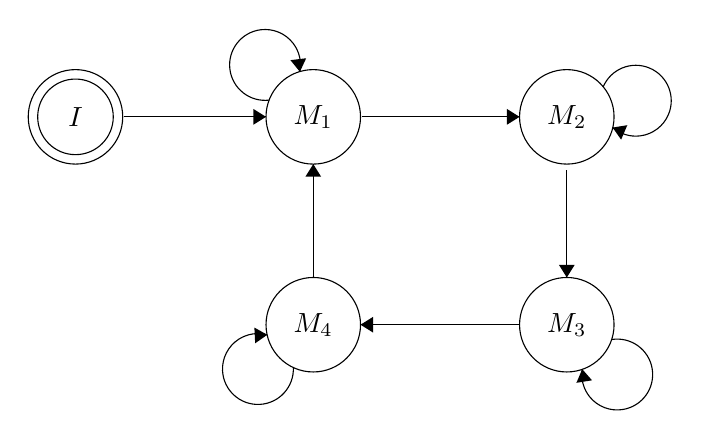
\begin{tikzpicture}[scale=0.2]

  \tikzstyle{every node}+=[inner sep=0pt]
  \draw [black] (6.7,-5.7) circle (3);
  \draw (6.7,-5.7) node {$I$};
  \draw [black] (6.7,-5.7) circle (2.4);
  \draw [black] (21.8,-5.7) circle (3);
  \draw (21.8,-5.7) node {$M_1$};
  \draw [black] (21.8,-18.9) circle (3);
  \draw (21.8,-18.9) node {$M_4$};
  \draw [black] (37.9,-5.7) circle (3);
  \draw (37.9,-5.7) node {$M_2$};
  \draw [black] (37.9,-18.9) circle (3);
  \draw (37.9,-18.9) node {$M_3$};
  \draw [black] (24.9,-5.7) -- (34.9,-5.7);
  \fill [black] (34.9,-5.7) -- (34.1,-5.2) -- (34.1,-6.2);
  \draw [black] (37.9,-9.1) -- (37.9,-15.9);
  \fill [black] (37.9,-15.9) -- (38.4,-15.1) -- (37.4,-15.1);
  \draw [black] (34.9,-18.9) -- (24.8,-18.9);
  \fill [black] (24.8,-18.9) -- (25.6,-19.4) -- (25.6,-18.4);
  \draw [black] (21.8,-15.9) -- (21.8,-8.7);
  \fill [black] (21.8,-8.7) -- (21.3,-9.5) -- (22.3,-9.5);
  \draw [black] (40.736,-19.842) arc (99.35081:-188.64919:2.25);
  \fill [black] (38.88,-21.72) -- (38.51,-22.59) -- (39.5,-22.43);
  \draw [black] (40.208,-3.802) arc (157.15825:-130.84175:2.25);
  \fill [black] (40.81,-6.38) -- (41.35,-7.15) -- (41.74,-6.23);
  \draw [black] (19.008,-4.636) arc (276.87022:-11.12978:2.25);
  \fill [black] (20.95,-2.84) -- (21.35,-1.98) -- (20.35,-2.1);
  \draw [black] (20.534,-21.607) arc (2.67649:-285.32351:2.25);
  \fill [black] (18.88,-19.54) -- (18.06,-19.08) -- (18.11,-20.08);
  \draw [black] (9.8,-5.7) -- (18.8,-5.7);
  \fill [black] (18.8,-5.7) -- (18,-5.2) -- (18,-6.2);

\end{tikzpicture}

        \caption{\Gls{FiniteStateMachine} veranschaulicht\label{fig:ConceptEngineFSM}}
      \end{figure}

      Aufgrund der Schnittstellen und bereits vorhandener Funktionen in der \gls{PhysicsEngine} ist ein Motor,
      der \gls{JointDriven} arbeitet gewählt worden.
      Er führt die Bewegungen, die Körperteile in Bewegung setzten, über die Drehgelenke des Individuums aus.
      Mit der Kraft des Motors wird der Winkel eines Drehgelenkes verändert.
      \\
      \\
      Am Beispiel des Kniegelenks ist ersichtlich wie der Motor arbeitet.
      Das Kniegelenk ist am Oberschenkel fixiert und verbindet den Unterschenkel mit dem Oberschenkel.
      Setzt der Motor das Gelenk in Bewegung wird der Unterschenkel bewegt.
      \\
      \\
      Mit den Informationen des Phänotyps kann der Motor den gesamten Bewegungsablauf kontrollieren.
      Der Motor überwacht die Übergänge zwischen den Bewegungen.
      Nach jedem Übergang zu einer neuen Bewegung, führt der Motor diese aus und prüft,
      ob der Zustand gewechselt werden muss.
      Ein Zustandswechsel ist gleichzusetzten mit einer neuen Bewegung auszuführen.

      \subsubsection{Ausführung in der Simulation}

        Die \gls{PhysicsEngine} führt die Simulation iterativ durch.
        D.h.\ der Zustand der Objekte in der Simulationswelt wird pro Schritt berechnet.
        Diese Eigenschaft nutzt der Motor,
        indem in während jedem Schritt die aktuelle Bewegung aller Individuen bearbeitet.
        Damit ist die feinst mögliche Auflösung für die Bewegungssteuerung erreicht.
        \\
        Als erstes bringt der Motor ein Individuum immer in die Ausgangsposition (\vref{fig:ConceptMovement00}).
        Die Ausgangsposition wird definiert durch den initialen Bewegungsablauf.
        Dieser ist unabhängig vom Ablauf, der das Gehen (oder eine andere Form der Fortbewegung) definiert.
        Sobald die Ausgangsposition erreicht ist, beginnt der Motor mit dem Ausführen des Bewegungsablaufs.

    \subsection{Vorgegebener Bewegungsablauf}

      Die Individuen der initialen Population~\vref{sec:initPop} besitzen einen vorgegebenen Bewegungsablauf.
      Der Grund dafür ist, dass damit die Wahrscheinlichkeit steigt,
      dass die Evolution lauffähige Individuen hervorbringt.
      \\
      Der vorgegebene Ablauf ist der Ameise nachempfunden, wegen der Einfachheit und Stabilität.
      Eine Ameise bewegt pro Schritt immer 3 Beine.
      Alternierend wird auf einer Seite 1 und auf der anderen 2 Beine gehoben und nach vorne bewegt.
      Diese Bewegung erlaubt es der Ameise stets stabil zu stehen,
      da ein Dreibein immer steht während die anderen bewegt werden.
      \\
      Mit dem vorgegebenen Muster werden die Bewegungen für eine Seite erstellt.
      Anschliessend können die Bewegungen für die andere Körperseite mit kleinen Anpassungen übernommen werden.

      \begin{enumerate}

        \setcounter{enumi}{-1}

        \item Der Motor setzt die Beine und Gelenke in ihre Ausgangsposition (\vref{fig:ConceptMovement00})

        \item In der ersten Phase werden die Beine der linken Seite bis zum maximalen Winkel bewegt
          (\vref{fig:ConceptMovement10}).

        \item Alle rechten Beine schieben nun den Körper nach vorne (\vref{fig:ConceptMovement15}) bis der minimale
          Winkel des Hüftgelenks erreicht wurde (\vref{fig:ConceptMovement20}).

        \item Die linken Beine werden nun gestreckt (\vref{fig:ConceptMovement30}).

        \item Anschliessend werden die rechten Beine nach vorne bewegt
          (\vref{fig:ConceptMovement35} und (\vref{fig:ConceptMovement36}))
          bis zum maximalen Winkel (\vref{fig:ConceptMovement40}).
          Der Bewegungsablauf wird gespiegelt für die Beine der anderen Körperseite vollzogen.

      \end{enumerate}

      \begin{figure}[H]
        \centering

        \begin{subfigure}[b]{0.3\textwidth}
          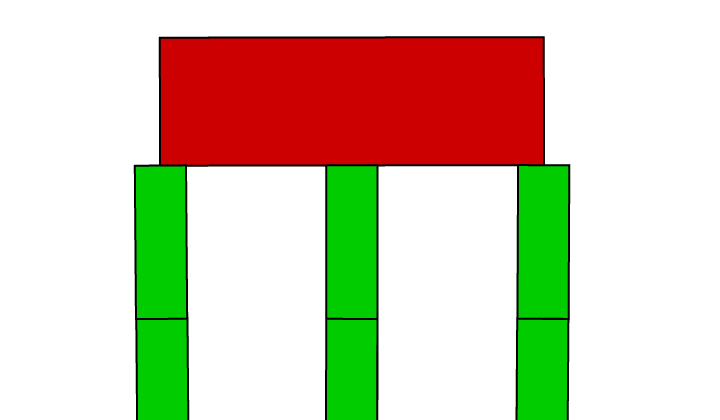
\includegraphics[width=\linewidth,center]{graphics/movement/00}
          \caption{\label{fig:ConceptMovement00}}
        \end{subfigure}
        \hspace{\fill}
        \begin{subfigure}[b]{0.3\textwidth}
          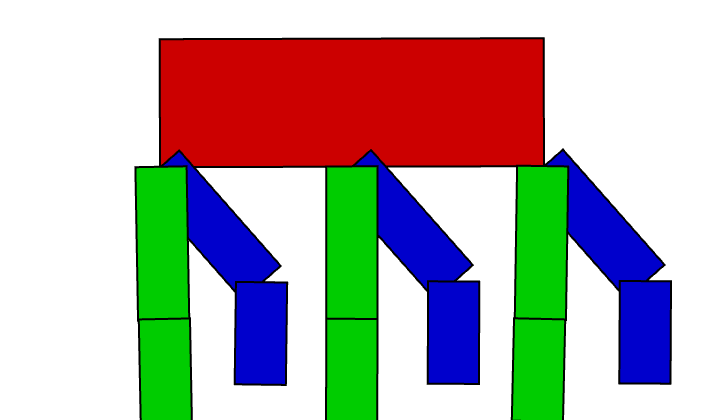
\includegraphics[width=\linewidth,center]{graphics/movement/05}
          \caption{\label{fig:ConceptMovement05}}
        \end{subfigure}
        \hspace{\fill}
        \begin{subfigure}[b]{0.3\textwidth}
          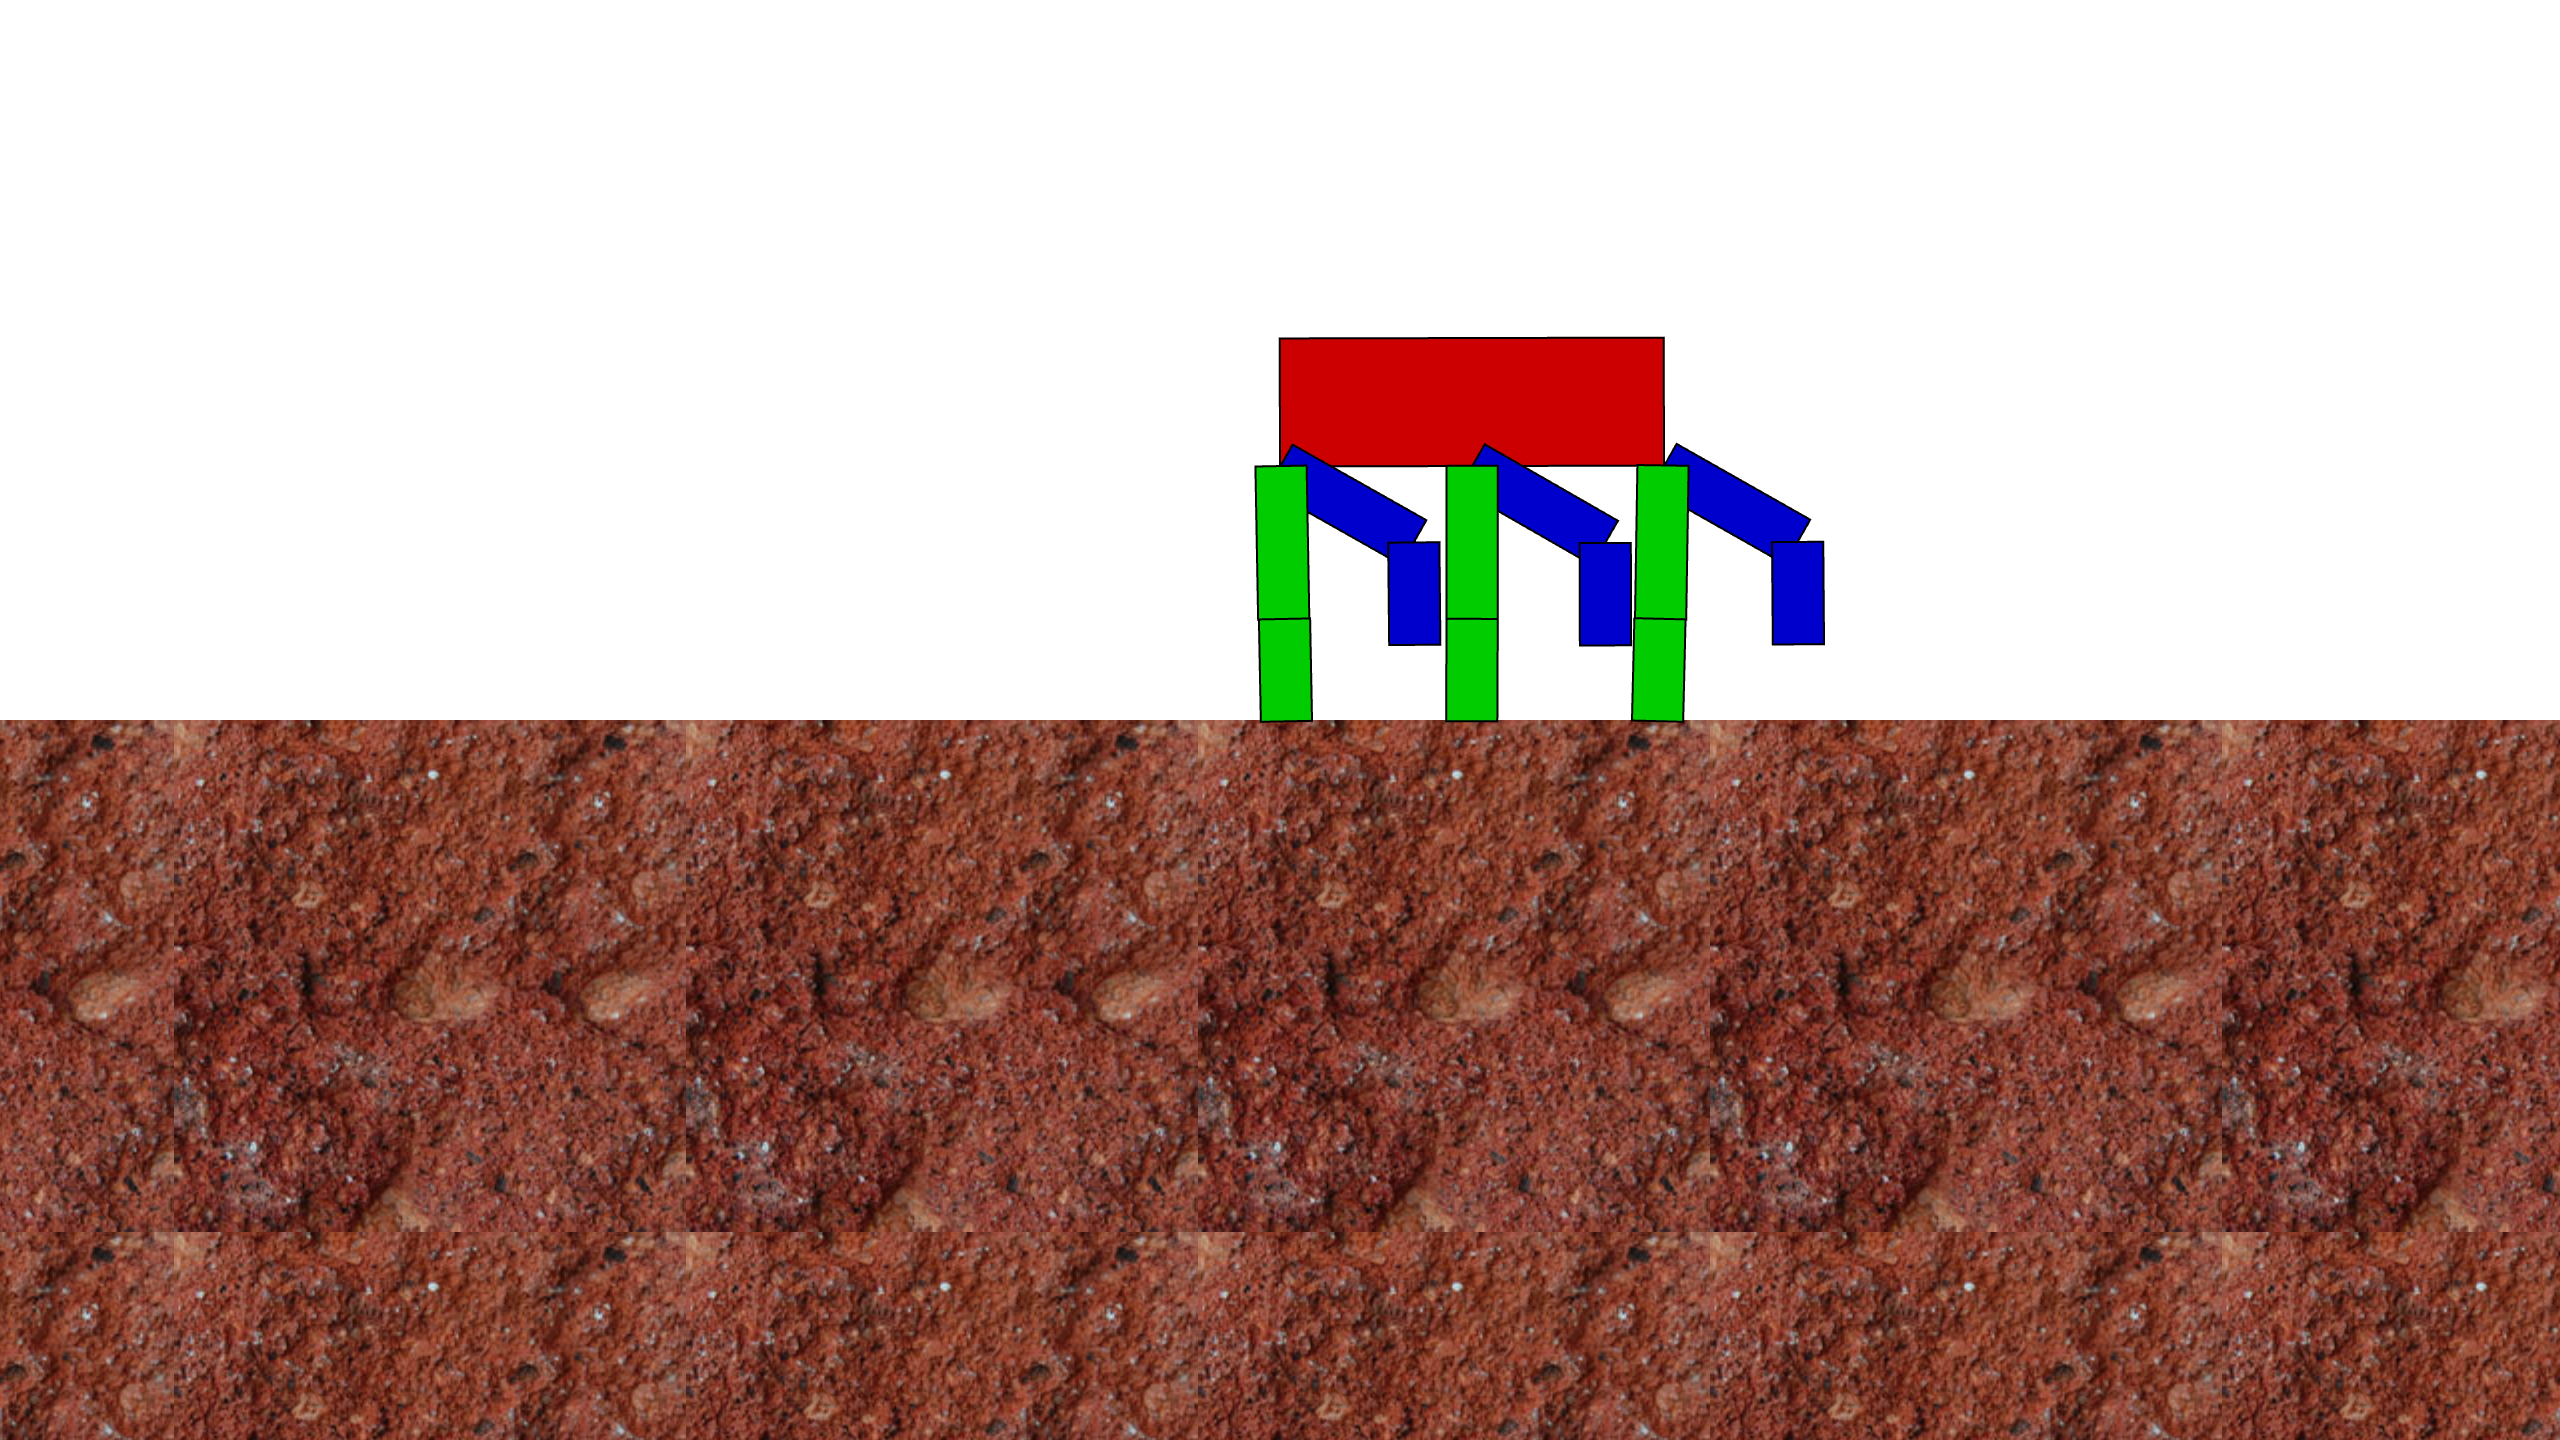
\includegraphics[width=\linewidth,center]{graphics/movement/10}
          \caption{\label{fig:ConceptMovement10}}
        \end{subfigure}

        \begin{subfigure}[b]{0.3\textwidth}
          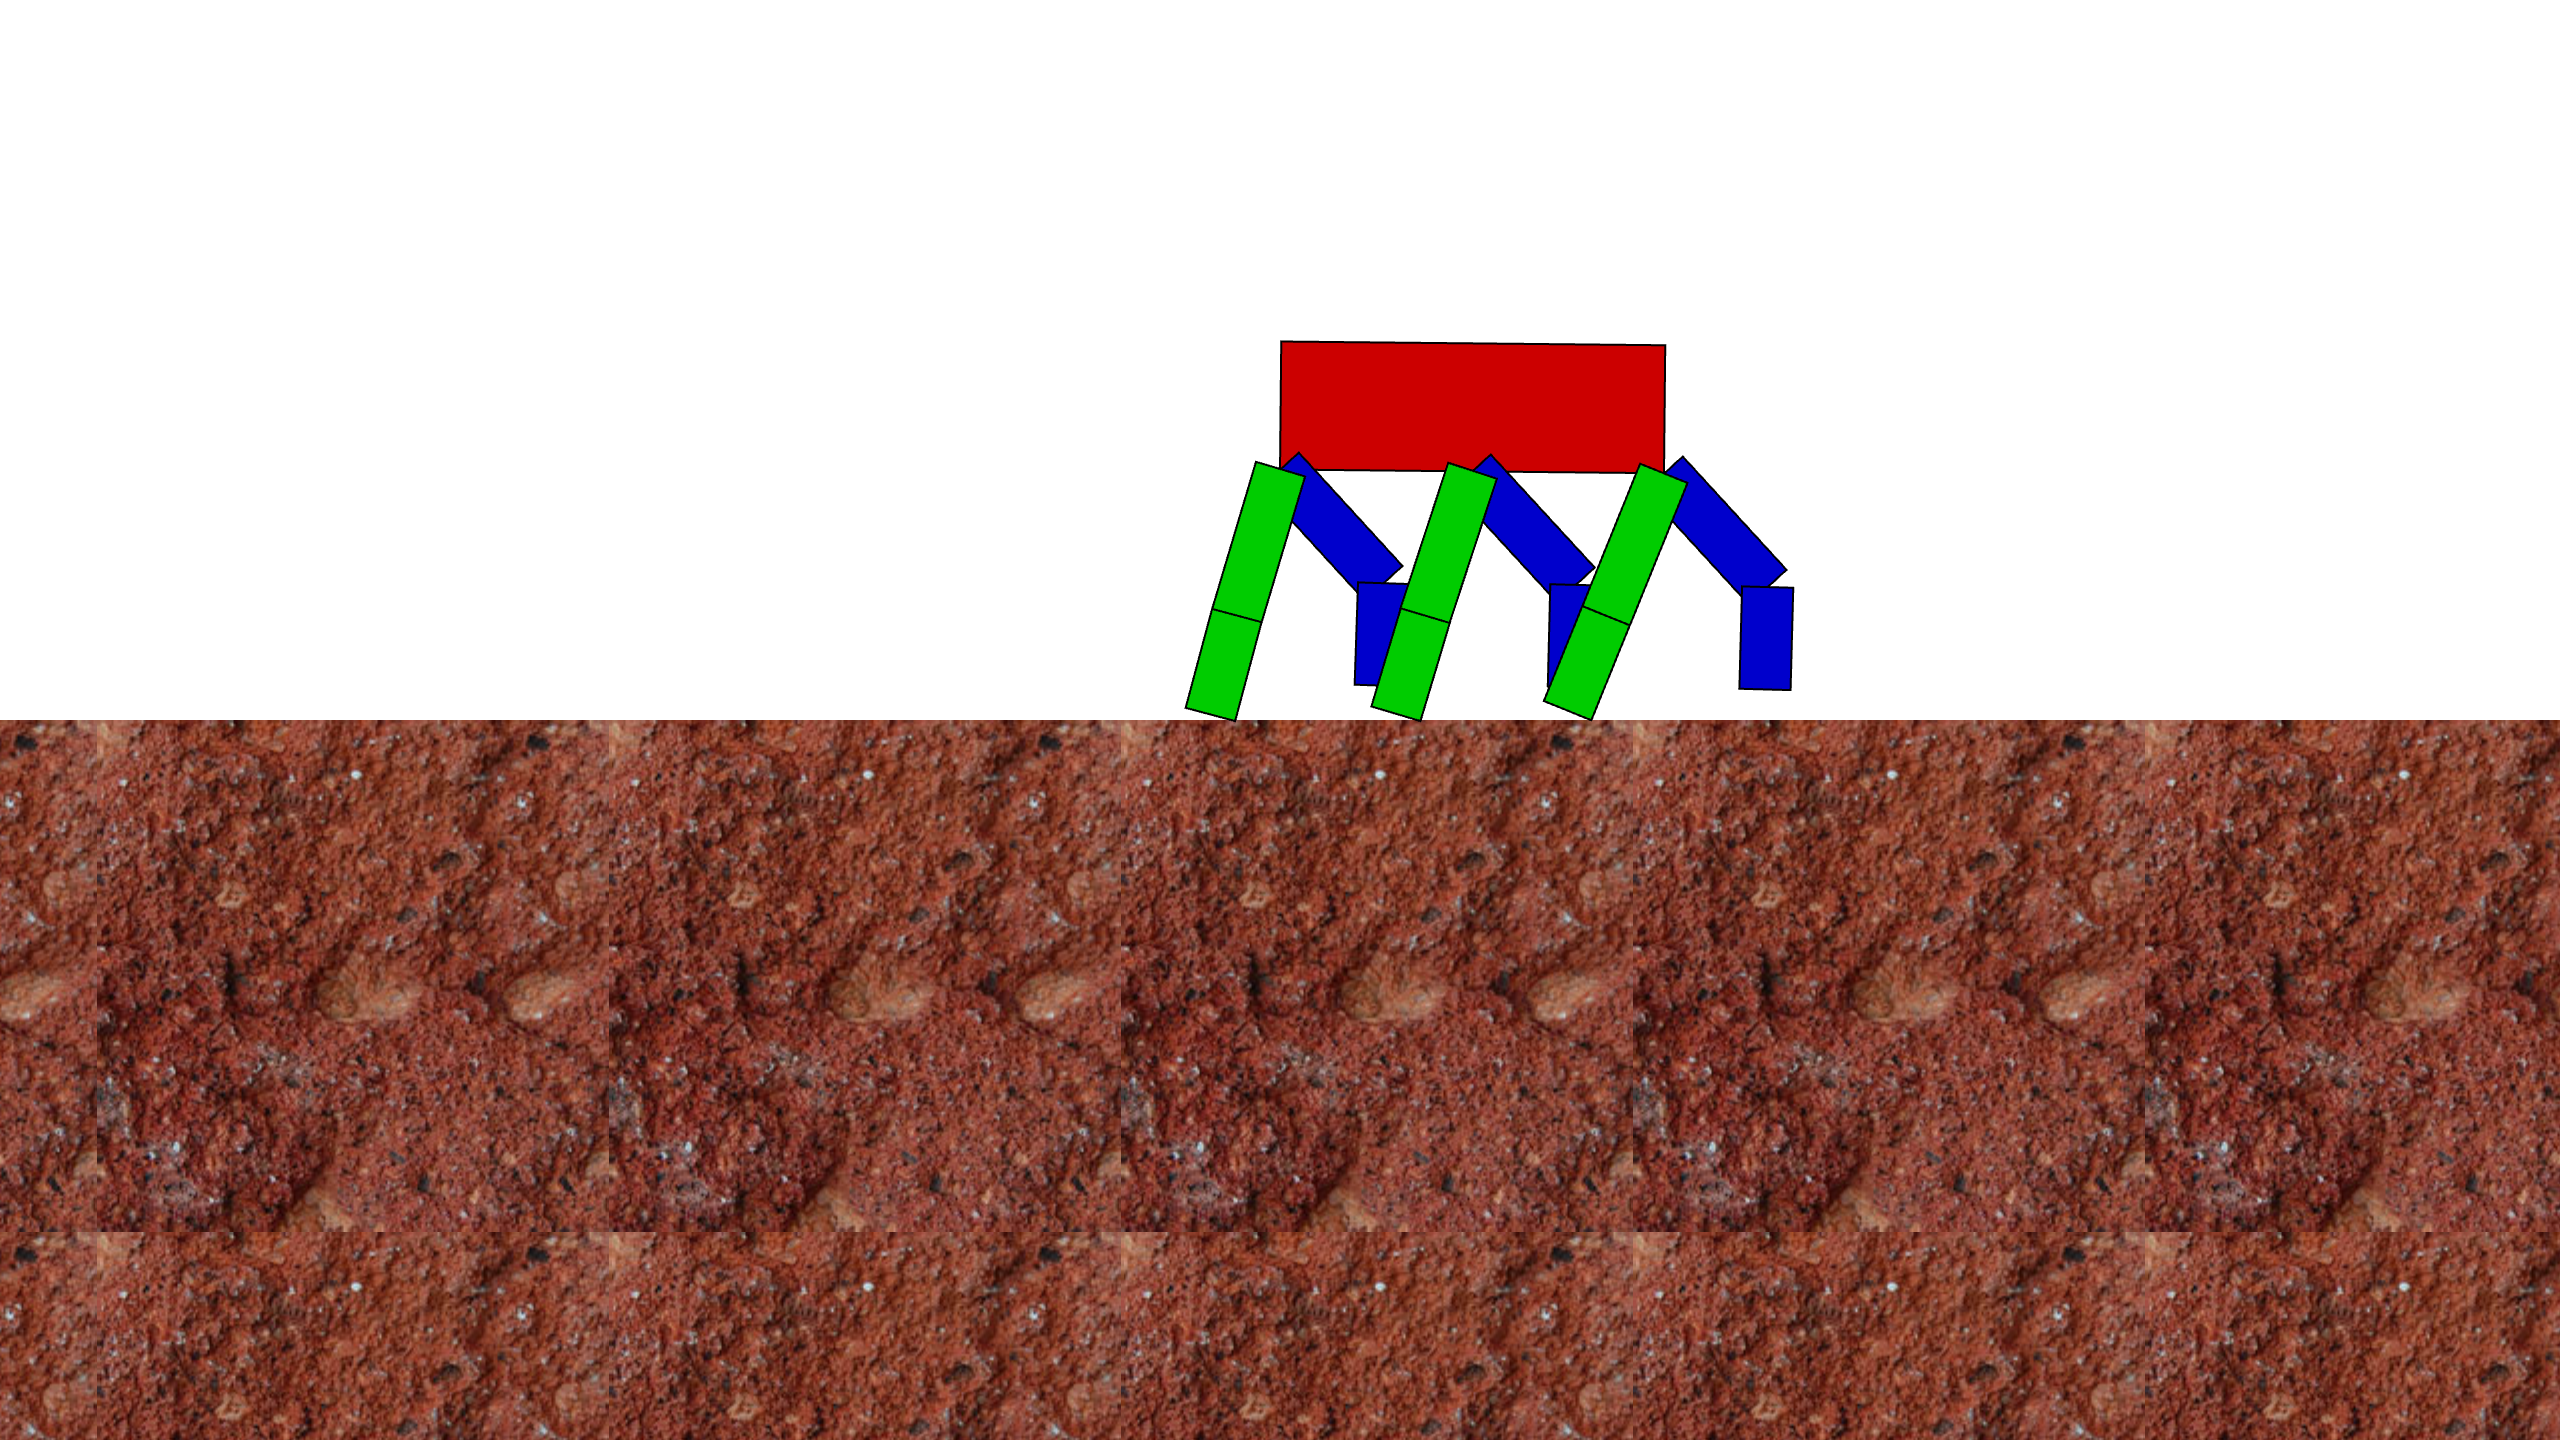
\includegraphics[width=\linewidth,center]{graphics/movement/15}
          \caption{\label{fig:ConceptMovement15}}
        \end{subfigure}
        \hspace{\fill}
        \begin{subfigure}[b]{0.3\textwidth}
          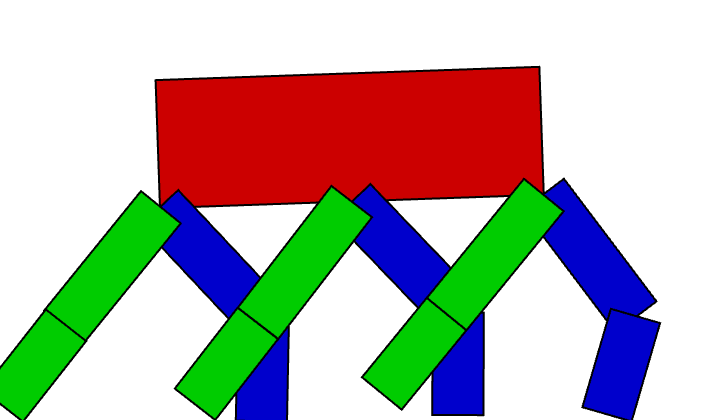
\includegraphics[width=\linewidth,center]{graphics/movement/20}
          \caption{\label{fig:ConceptMovement20}}
        \end{subfigure}
        \hspace{\fill}
        \begin{subfigure}[b]{0.3\textwidth}
          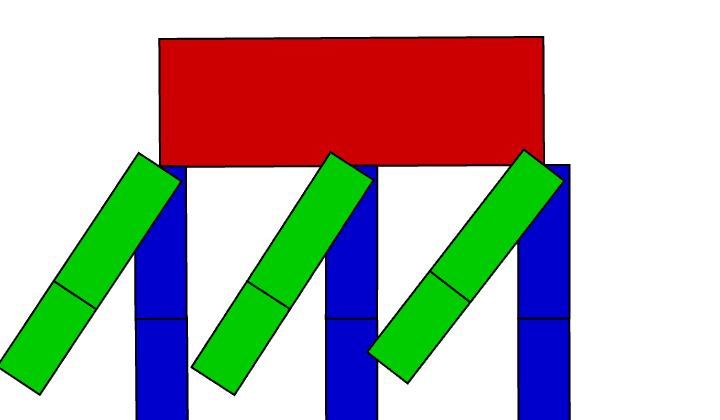
\includegraphics[width=\linewidth,center]{graphics/movement/30}
          \caption{\label{fig:ConceptMovement30}}
        \end{subfigure}

        \begin{subfigure}[b]{0.3\textwidth}
          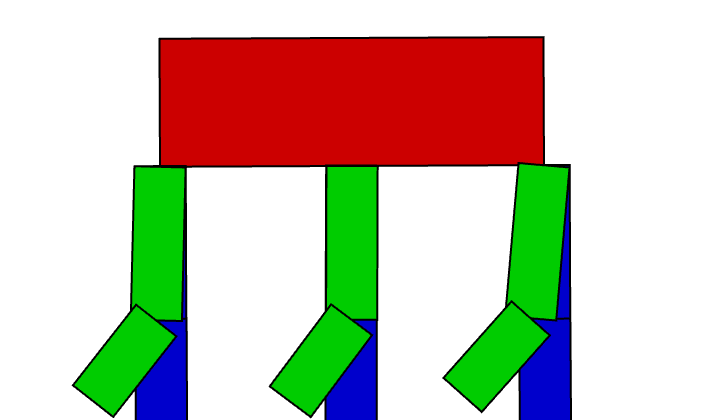
\includegraphics[width=\linewidth,center]{graphics/movement/35}
          \caption{\label{fig:ConceptMovement35}}
        \end{subfigure}
        \hspace{\fill}
        \begin{subfigure}[b]{0.3\textwidth}
          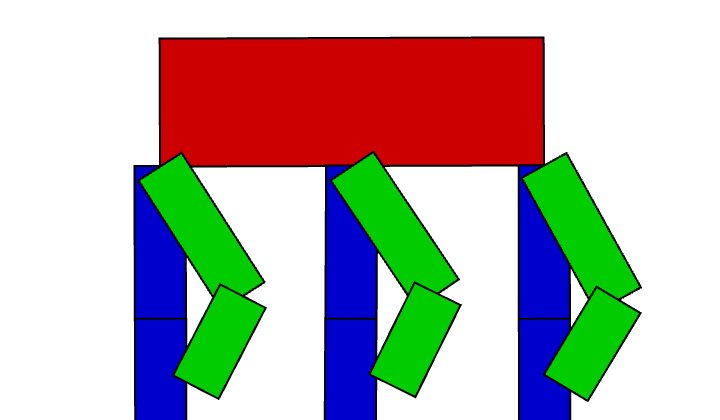
\includegraphics[width=\linewidth,center]{graphics/movement/36}
          \caption{\label{fig:ConceptMovement36}}
        \end{subfigure}
        \hspace{\fill}
        \begin{subfigure}[b]{0.3\textwidth}
          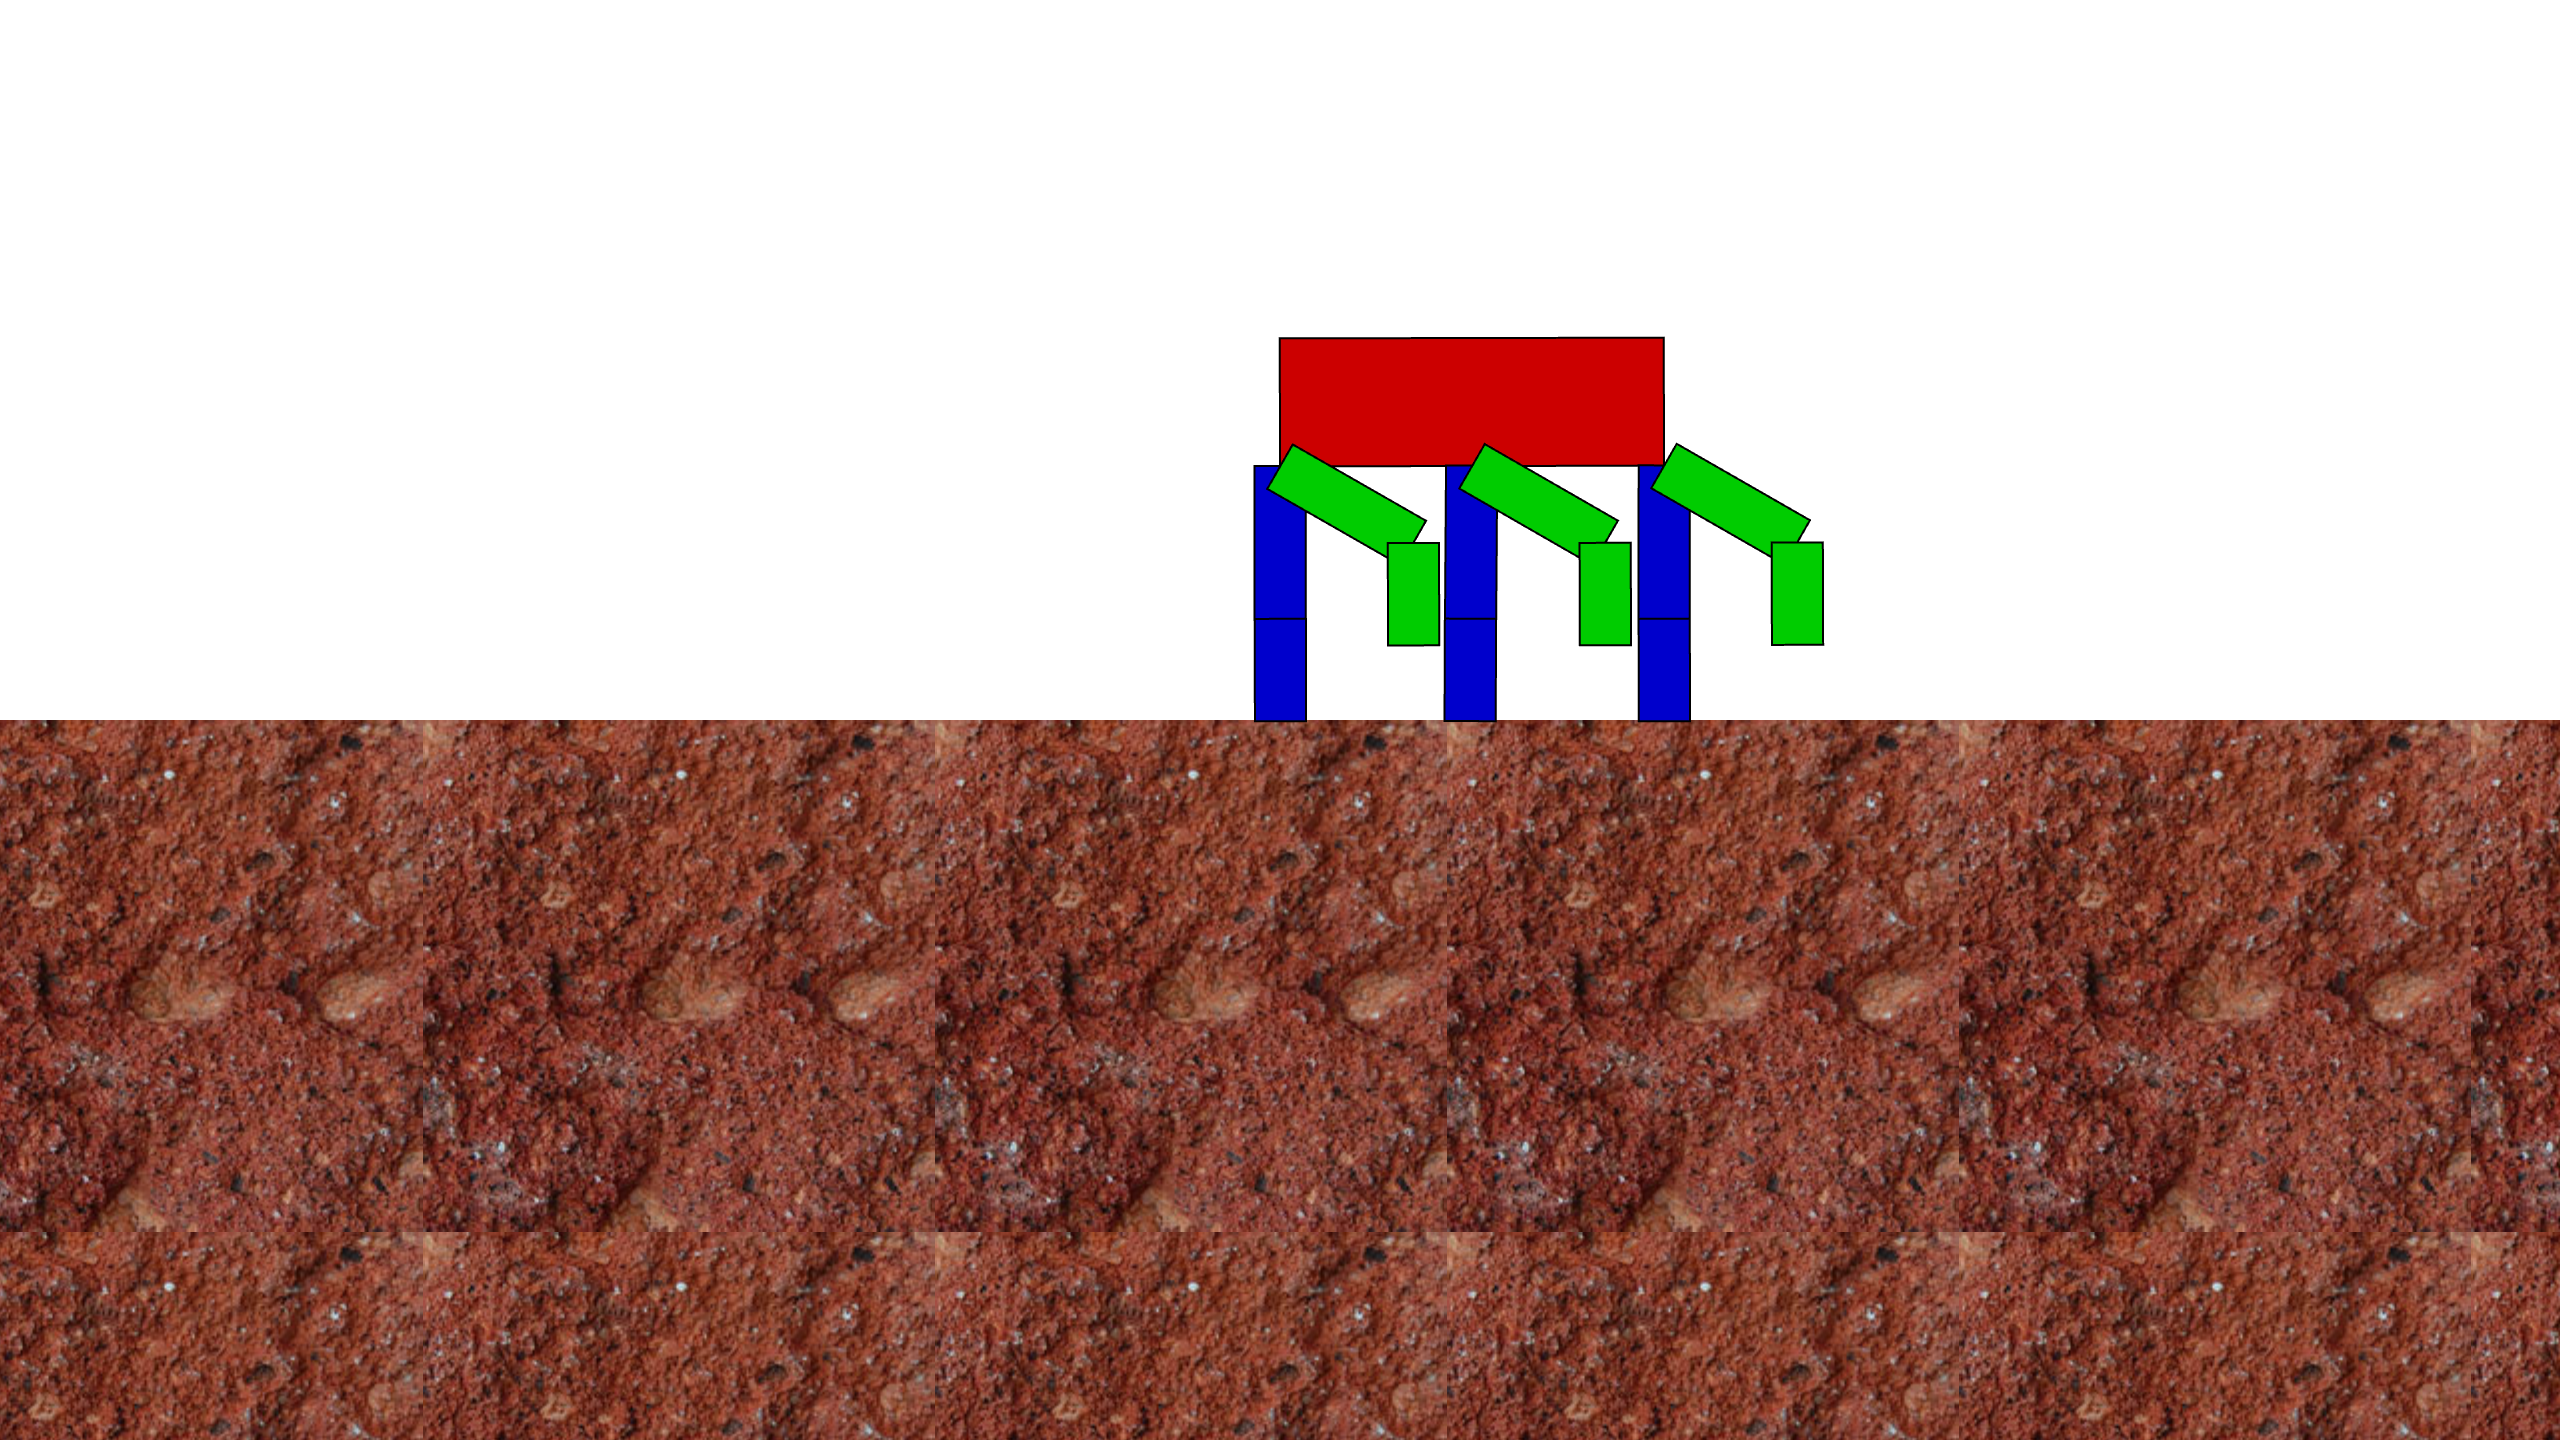
\includegraphics[width=\linewidth,center]{graphics/movement/40}
          \caption{\label{fig:ConceptMovement40}}
        \end{subfigure}

        \begin{subfigure}[b]{0.3\textwidth}
          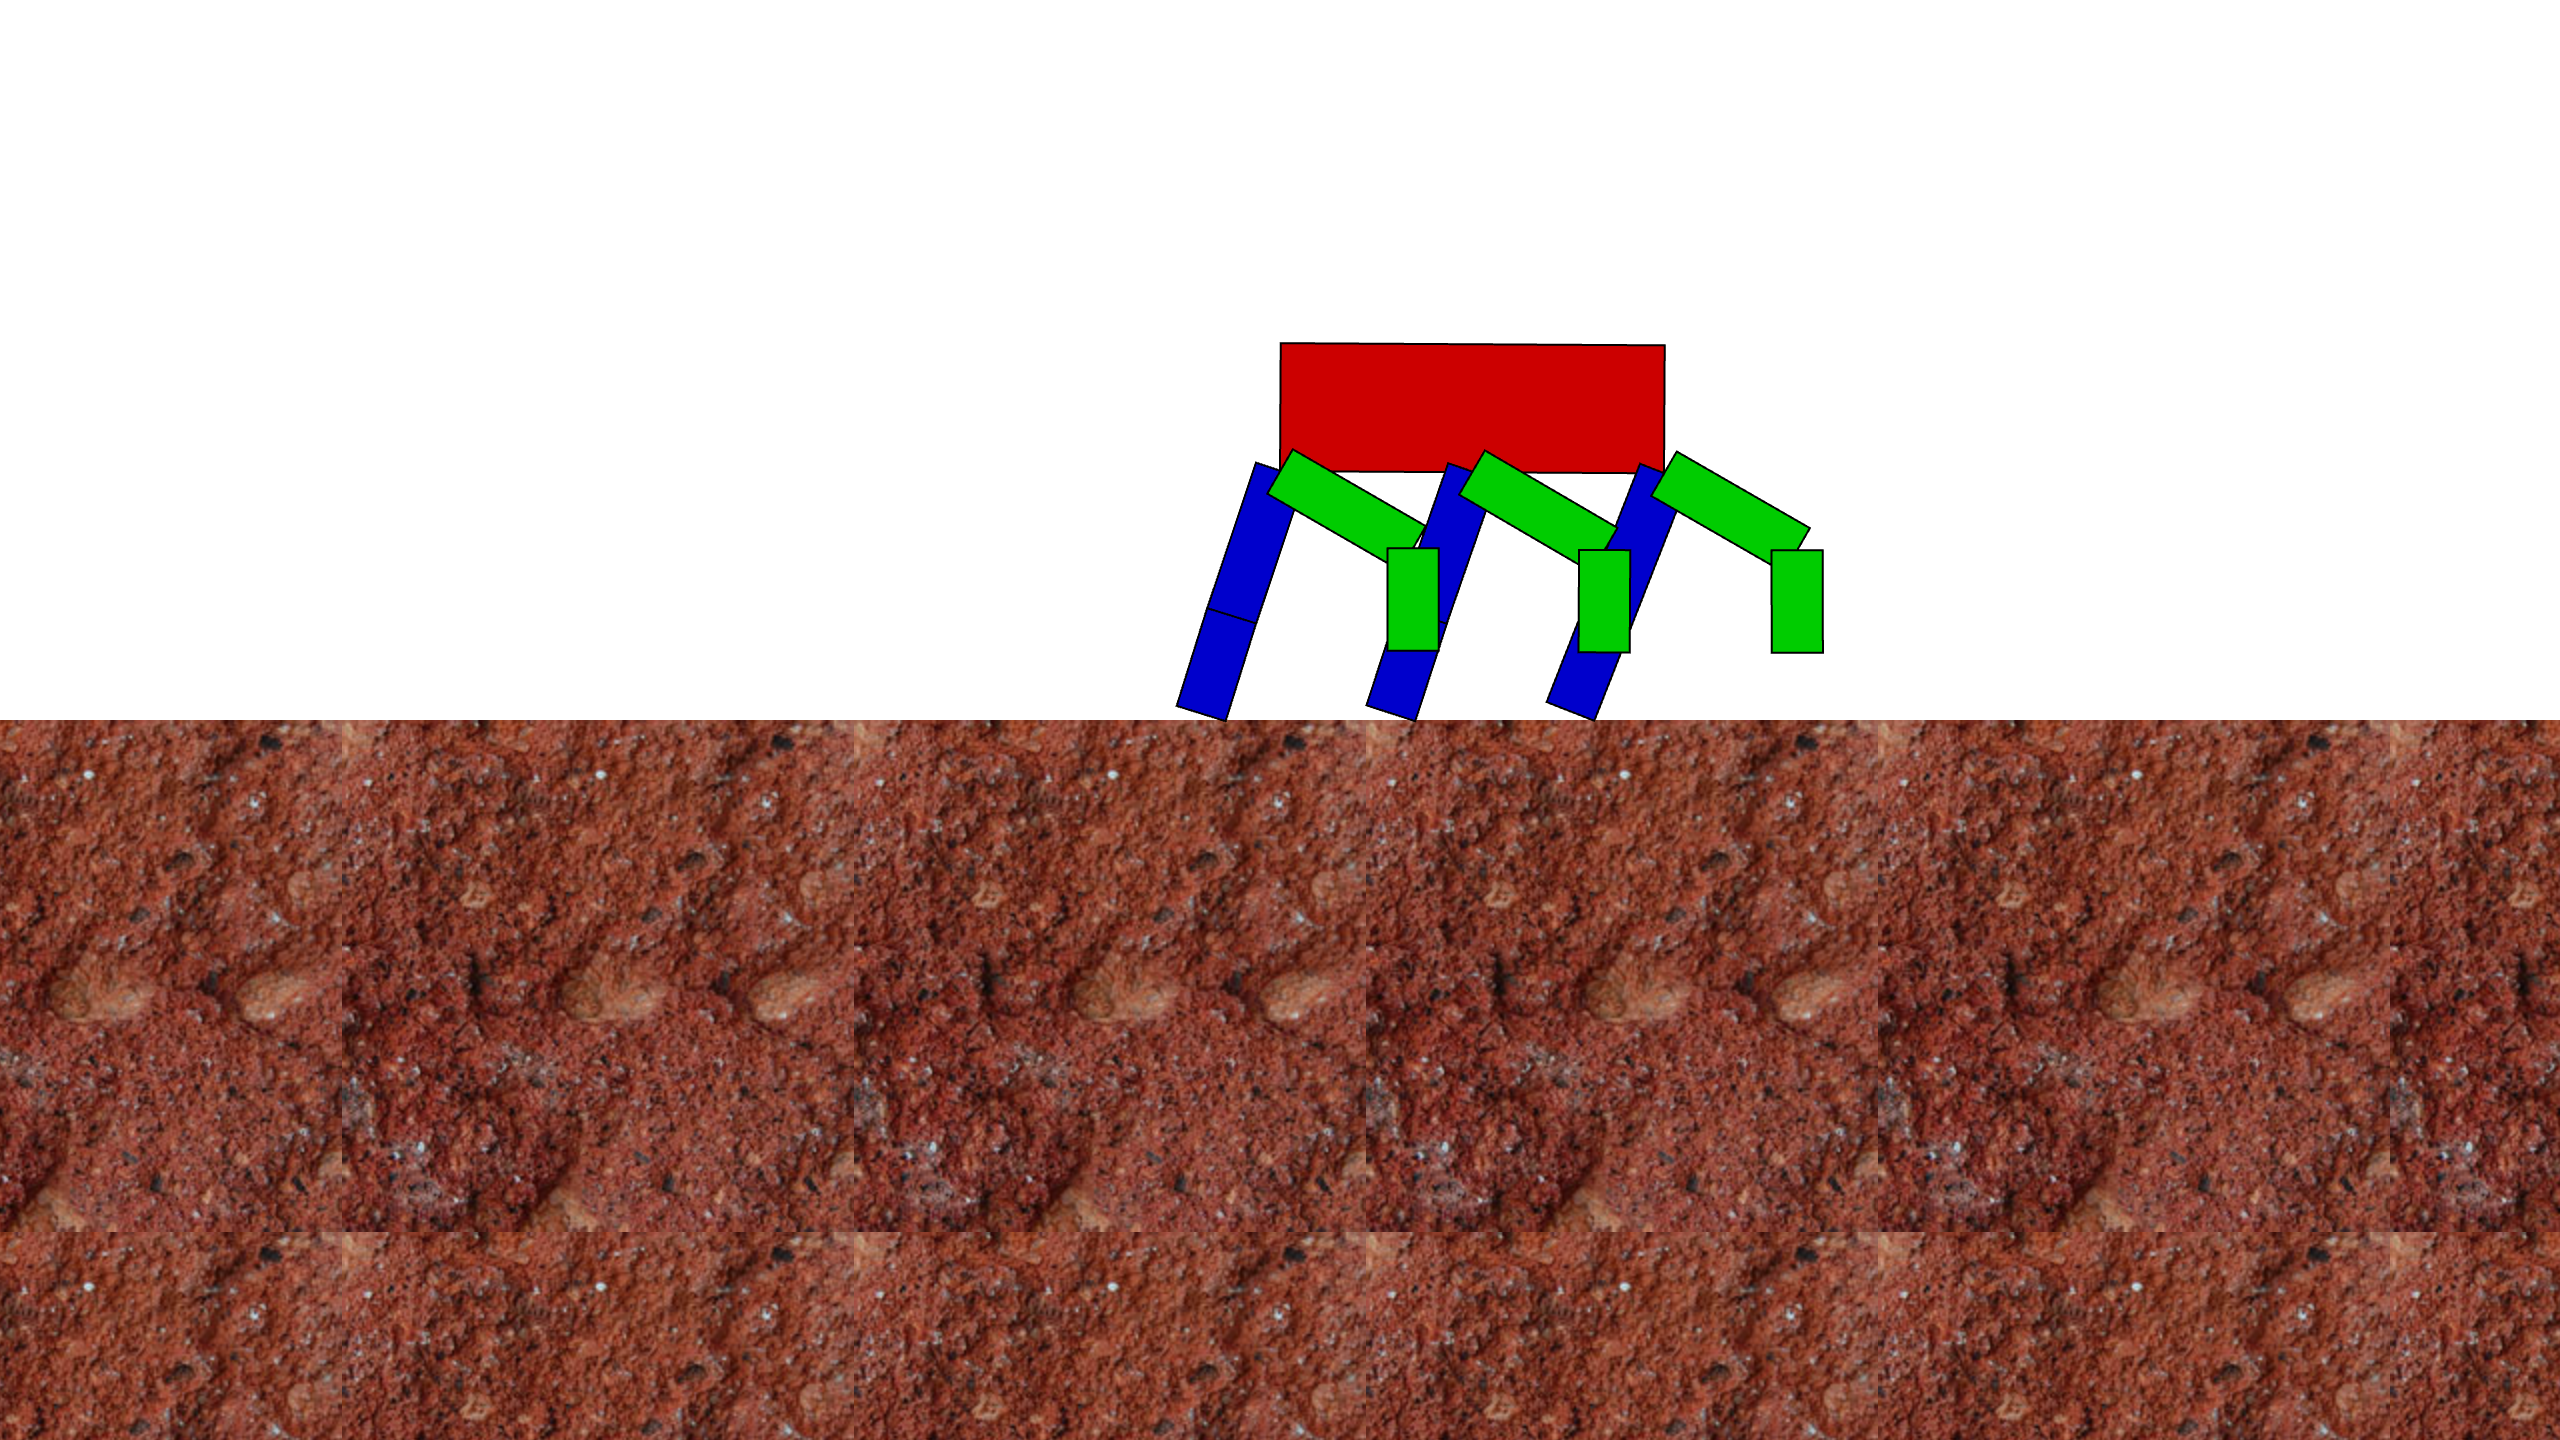
\includegraphics[width=\linewidth,center]{graphics/movement/45}
          \caption{\label{fig:ConceptMovement45}}
        \end{subfigure}
        \hspace{\fill}
        \begin{subfigure}[b]{0.3\textwidth}
          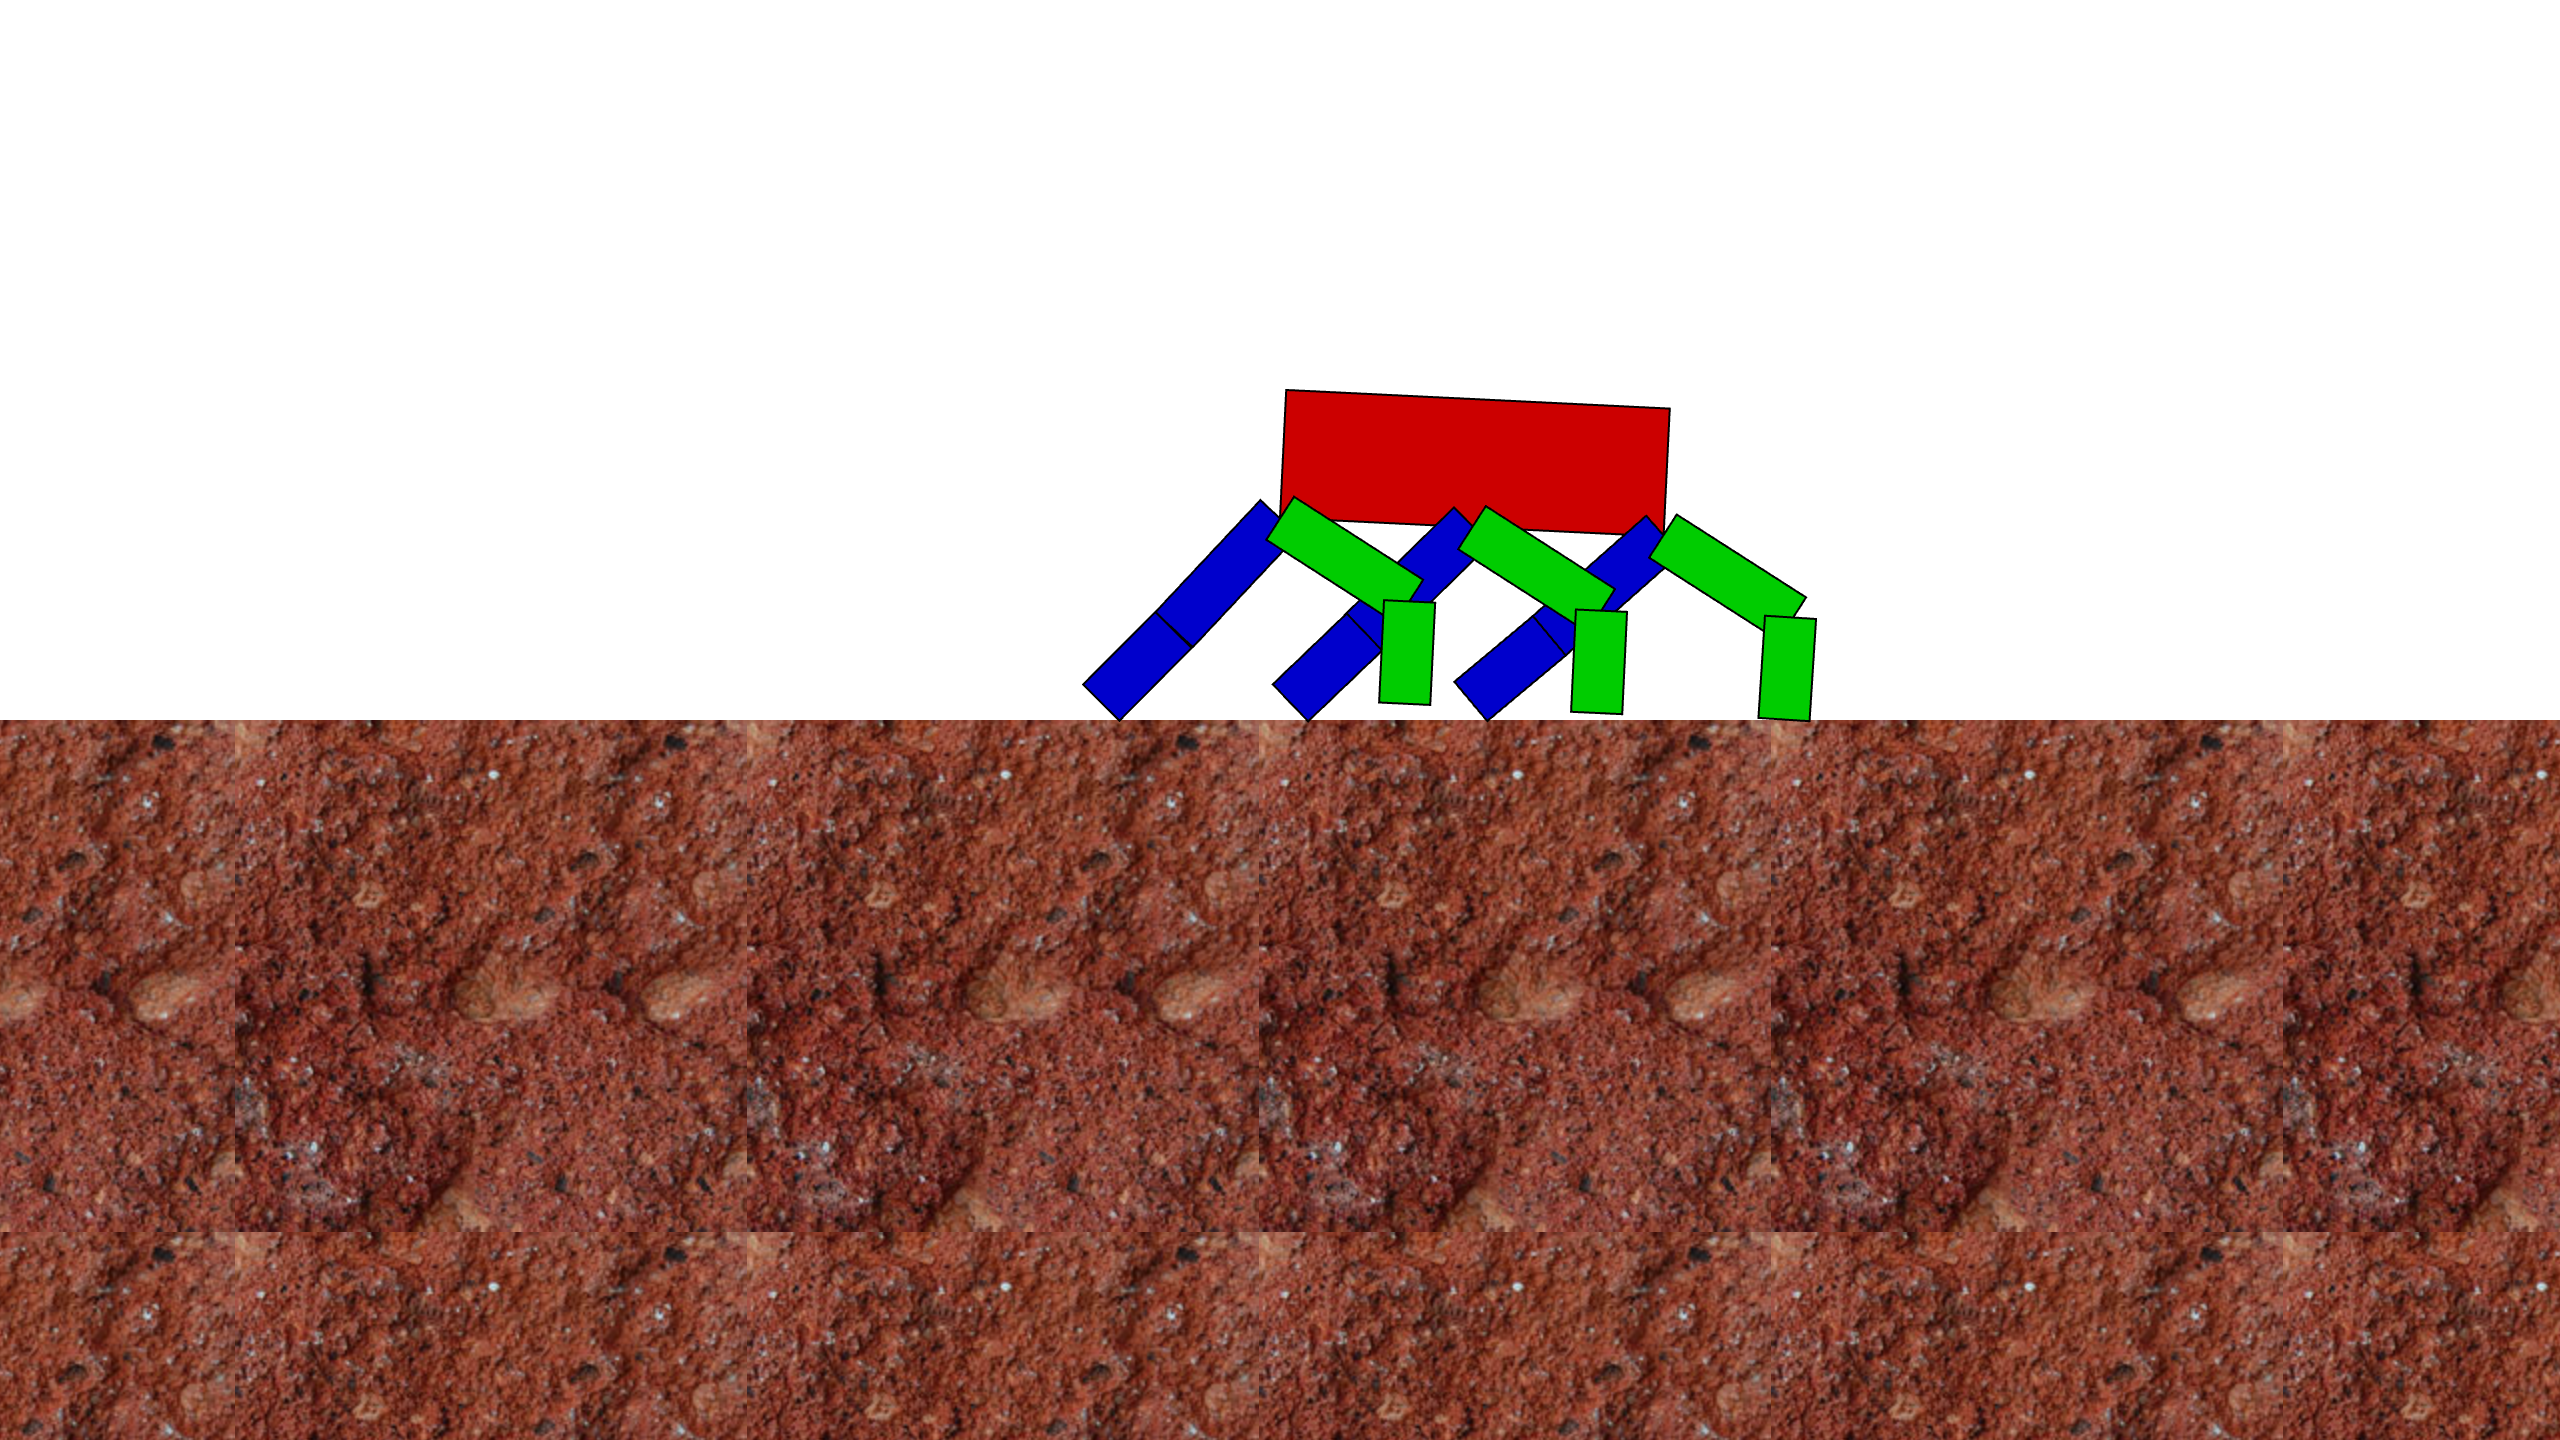
\includegraphics[width=\linewidth,center]{graphics/movement/50}
          \caption{\label{fig:ConceptMovement50}}
        \end{subfigure}
        \hspace{\fill}
        \begin{subfigure}[b]{0.3\textwidth}
          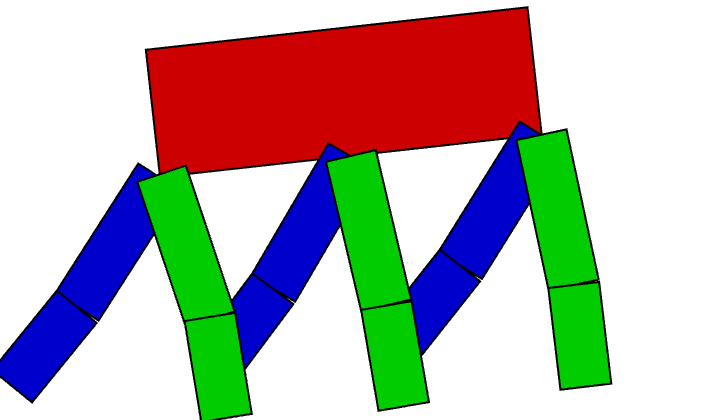
\includegraphics[width=\linewidth,center]{graphics/movement/55}
          \caption{\label{fig:ConceptMovement55}}
        \end{subfigure}

        \caption{Bewegungsablauf im Zeitraffer\label{fig:ConceptMovement}}

      \end{figure}

      \subsubsection{Bewegung\label{subsub:EngineMovement}}

        Unter dem Begriff Bewegung werden alle Aktionen, die der Motor ausführt verstanden.
        Es gibt neben den klassischen Bewegungen, wie ein Drehgelenk bewegen,
        auch solche, die Attribute eines Gelenkes ändern oder den aktuellen Winkel eines Gelenkes abfragen.
        \\
        \\
        Eine Bewegung ist mit mehreren Attributen beschrieben.
        Es wird festgelegt welche Art der Bewegung es ist,
        welches Gelenk gesteuert wird und was die Parameter für die Bewegung sind.
        Mit dieser Aufgliederung lassen sich einzelne Teile einer Bewegung mutieren.
        Insbesondere ist es möglich verschiedene Wahrscheinlichkeiten für Teile zu verwenden.
        \\
        Sobald der Motor eine Bewegung ausführt, interpretiert er die Daten aus dem Phänotyp.
        Er liest die Beschreibung der aktuellen Bewegung und führt diese dann aus.

      \subsubsection{Feedback}

        Zur weiteren Verbesserung des Bewegungsablaufs,
        kann der Motor Rückmeldungen von der Simulationswelt anfordern.
        Der Motor wird von der \gls{PhysicsEngine} benachrichtigt,
        sobald eine Kollision zwischen einem Körperteil und dem Untergrund stattfindet.
        \\
        \\
        Das Feedbacksystem ist nicht vollständig ausgearbeitet.
        Aus zeitlichen Gründen ist dies nicht umgesetzt worden.
        Es ist nur die Rückmeldung an den Motor vorhanden, jedoch wird die Rückmeldung nicht verarbeitet.
        Im Kapitel~\vref{sec:PerspectiveFeedback} wird erläutert, was zusätzlich umgesetzt werden muss.

  \section{Auswahl des evolutionären Algorithmus}

    Es stehen 4 Typen von evolutionären Algorithmen zur Auswahl:

    \begin{itemize}
      \item Genetische Algorithmen~(GA)~(\vref{item:genAlgo})
      \item Genetische Programmierung~(GP)~(\vref{item:genProg})
      \item Evolutionäre Programmierung~(EP)~(\vref{item:evProg})
      \item Evolutionäre Strategien~(ES)~(\vref{item:evStrat})
    \end{itemize}

    % TODO umformulieren

    %Um die Problemstellung zu lösen, wurde entschieden Evolutionäre Programmierung einzusetzen
    Das Austauschen der Gene (Rekombination) ist wenig hilfreich bei der Lösung der Problemstellung.
    Man stelle sich dazu vor, dass das Gen welches den Körper definiert, mit dem des Motors vertauscht wird.
    So kann keine sinnvolle Evolution statt finden.
    Rekombination kann für die Verwendung somit ausgeschlossen werden.
    Dies stellt schon den ersten Indikator dar,
    dass Evolutionäre Programmierung eingesetzt werden kann.
    Ein weiteres Kriterium ist die genetische Repräsentation.
    Da sich das Individuum aus Punkten im einem Koordinatensystem,
    verschiedene Winkel und einem Antrieb (Motor) definiert, wird die Reale-Werte-Repräsentation eingesetzt.
    Ein Punkt ist nichts anderes als zwei reale Werte,
    ein Winkel kann ebenfalls so beschrieben werden und ein Antrieb auch.
    Die binäre Repräsentation scheint für die vielen realen Werte nicht geeignet zu sein.
    Theoretisch wäre es möglich alle reale Werte binär darzustellen, jedoch würde so dem Problem eine unnötige Komplexität hinzugefügt werden.
    Die Repräsentation als Baum ist laut K. Weicker~\cite{book:evAlgo} eine Möglichkeit die Steuerung eines Roboters abzubilden.
    Da aber mehr als nur die Steuerung evolviert wird, bleibt die Entscheidung bei der Reale-Werte-Repräsentation.
    Die Problemstellung würde wahrscheinlich anders bewältigt werden,
    würde sich die Thematik um reale Kreaturen drehen und nicht um virtuelle Roboter,
    welche in einer künstlichen Umgebung (virtuelles Koordinatensystem) das Laufen lernen.
    Bei realen Kreaturen spielt die Genetik eine zentrale Rolle, jedoch kann sie bei den virtuellen Robotern vernachlässigt werden.
    Schlussendlich wurde entschieden die Problemstellung, aufgrund der gelieferten Argumente, mit evolutionärer Programmierung zu lösen.

  \section{Eingesetzte Technologien\label{sec:Technology}}

    Zur Auswahl standen mehrere Programmiersprachen und \glspl{PhysicsEngine}.
    Die Evaluationskriterien dabei waren:

    \begin{itemize}
      \item Plattform-Interoperabilität (Linux, Windows und Mac OS X)
      \item Einfache Handhabung
      \item Stabilität
      \item Funktionsumfang der \gls{PhysicsEngine}
      \item Ökosystem der Programmiersprache (verfügbare Bibliotheken)
    \end{itemize}

    Als erstes wurde \gls{FSharp} und diverse populäre \gls{DotNet} \glspl{PhysicsEngine} wie ``Farseer Physics'',
    ``Physics 2D'' und ``Digital Rune Engine'' evaluiert.
    Jedoch gestaltete sich die Konfiguration und Plattform-Interoperablität schwierig.
    Eine plattformübergreifende Konfiguration, konnte nicht erstellt werden.
    Dies lag nicht an den \glspl{PhysicsEngine}, sondern an der Open-Source-Implementation von ``Mono Game''.
    ``Mono Game'' und Mono werden verwendet, um die \gls{DotNet}-Umgebung auf Linux und Mac zu nutzen.
    \\
    \\
    Als zweite Möglichkeit wurde Javascript und die \glspl{PhysicsEngine} ``Matter.js'' und ``p2.js'' in Betracht gezogen.
    Die Popularität von Javascript hat in den letzten Jahren enorm zugenommen.
    Auch wurde mit dem neuen ECMA2015 Standard die Sprache enorm verbessert und viele neue Features eingeführt.
    Das Javascript-Ökosystem ist eines der grössten überhaupt.
    Da Javascript ursprünglich eine Webtechnologie ist und auf allen Plattformen problemlos läuft,
    wurde das Kriterium der Plattform-Interoperabilität ohne zusätzliche Konfiguration erfüllt.

    \subsection{Auswahl der \gls{PhysicsEngine}}

      Im Zentrum der Anwendung steht die \gls{PhysicsEngine}, welche die ganze Simulation berechnet.
      Für die Auswahl der \gls{PhysicsEngine} war es besonders wichtig,
      dass diese die notwendige Funktionalität bereitstellt.
      \\
      Die erste Option war ``Matter.js''. Schnell hat sich herausgestellt,
      dass diese \gls{PhysicsEngine} nicht genug ausgereift ist.
      Deshalb wurde als zweite Option auf ``p2.js'' zurückgegriffen.
      Diese \gls{PhysicsEngine} bietet eine ausführliche Dokumentation und Beispiele zu sämtlichen Aspekten.

    \subsection{Fehler in der \gls{PhysicsEngine}}

      Für die Erstellung des Terrains wird ein Höhenfeld von p2.js benutzt.
      Die Kollisionserkennung zwischen einem Höhenfeld und einem Polygon funktioniert nicht einwandfrei.
      Manche Polygonecken werden nicht berücksichtigt in der Kollisionserkennung.
      Das hat zur Folge, dass Körperteile der Individuen im Boden einsinken.
      \vref{fig:vorEinsinken} zeigt ein Individuum vor dem Einsinken
      und~\vref{fig:nachEinsinken} zeigt ein Individuum mit einer eingesunkenen Spitze.

      \begin{figure}[H]
        \centering
        \begin{subfigure}[b]{0.45\textwidth}
          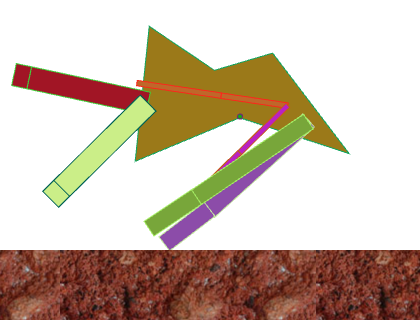
\includegraphics[width=\linewidth,center]{graphics/physics-engine/sink-0}
          \caption{Vor dem Einsinken\label{fig:vorEinsinken}}
        \end{subfigure}
        \qquad
        \begin{subfigure}[b]{0.45\textwidth}
          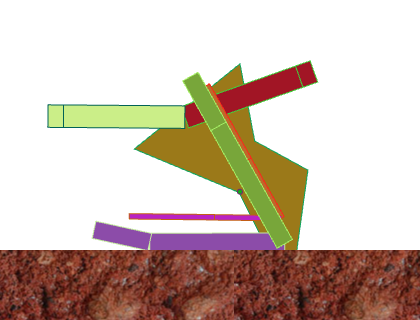
\includegraphics[width=\linewidth,center]{graphics/physics-engine/sink-1}
          \caption{Nach dem Einsinken\label{fig:nachEinsinken}}
        \end{subfigure}
        \caption{Vor Korrektur}
      \end{figure}

      Die Kollision mit einem Höhenfeld wird am besten erkannt mit einem Kreis.
      In~\vref{fig:noVorEinsinken} sind an allen Ecken des Körpers und der Beine kleine Kreise angebracht.
      Diese besitzen eine vernachlässigbare Masse, damit keine Nebeneffekte auftreten.
      Dies verbessert die Kollisionserkennung zwischen den Phänotypen und dem Untergrund.
      Wie in~\vref{fig:noNachEinsinken} erkennbar, sinkt die Spitze des Individuums nicht mehr in den Boden ein.
      Die zusätzlichen Objekte, welche für diese Optimierung verwendet wurden,
      erhöhen den Rechenaufwand der Simulation.

      \begin{figure}[H]
        \centering
        \begin{subfigure}[b]{0.45\textwidth}
          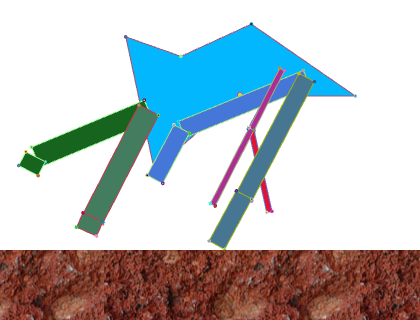
\includegraphics[width=\linewidth,center]{graphics/physics-engine/sink-fix-0}
          \caption{Individuum mit Kreisen\label{fig:noVorEinsinken}}
        \end{subfigure}
        \qquad
        \begin{subfigure}[b]{0.45\textwidth}
          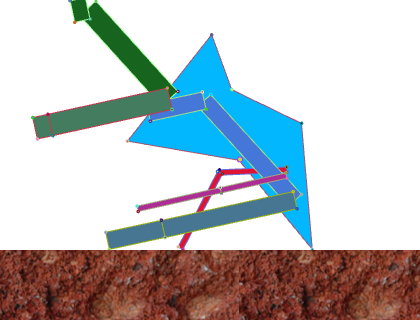
\includegraphics[width=\linewidth,center]{graphics/physics-engine/sink-fix-1}
          \caption{Verhindern des Einsinkens\label{fig:noNachEinsinken}}
        \end{subfigure}
        \caption{Nach Korrektur}
      \end{figure}

    \subsection{Laufzeitumgebung}

      % TODO umformulieren

      Um Javascript und p2.js ohne Browser zu betreiben, wird Electron eingesetzt.
      Electron ist node.js und Google Chrome vereint in einer Standalone-Anwendung.
      Mit Hilfe von Node.js lassen sich alle I/0-Zugriffe regeln und es kann auf den
      Node Package Manager zur Abhängigkeitsverwaltung von anderen Bibliotheken zurückgegriffen werden.
      Auch lässt sich unter bestimmten Umständen Javascript schneller ausführen unter Node.js als in einem Browser.

    % TODO ergänzen was wie wo oder löschen!
    \subsection{Programmierparadigma\label{sub:TechnologyParadigma}}

      In der Programmierung gibt es verschiedene Ansätze,
      wie der Quellcode aufgebaut werden soll und wie Probleme gelöst werden sollen.
      Die bekanntesten Ansätze sind prozedural, objektorientiert und funktional.

      \subsubsection{Prozedural\label{subsub:TechnologyParadigmaProzedural}}

        Prozedurale Programme bestehen aus einer Folge von Befehlen,
        die vorgeben wann was ausgeführt wird.
        Die Daten und die Routinen die mit diesen arbeiten, sind voneinander getrennt.

      \subsubsection{Objekt-Orientiert\label{subsub:TechnologyParadigmaObjectOriented}}

        Die objektorientierte Programmierung verbindet die Daten und
        die Routinen die mit diesen interagieren. Sie werden zu Einheiten zusammengefasst.
        Diese Einheiten werden im Zusammenhang mit Objekt-Orientierter-Programmierung Klassen genannt.

      \subsubsection{Funktional\label{subsub:TechnologyParadigmaFunctional}}

        Funktionale Programmierung heisst, das Programm so zu entwerfen,
        so dass die Datenverarbeitung nur aus Evaluationen von Funktionen besteht.
        Wenn Mutationen durchgeführt werden, wird anstatt die jeweilige Eigenschaft zu verändern,
        ein neues Objekt inklusive der Mutation zurückgegeben.
        Ohne mutable State ist es einfach Parallelisierung zu implementieren. % TODO glossar
        Es wird anstatt Iterationen, Rekursionen verwendet.
        In der funktionalen Programmierung versucht man Funktionen die Nebeneffekte haben (globale Attribute) zu vermeiden.
        Dies hat den Vorteil, dass einzelne Funktionen viel einfacher zu testen sind,
        als bei der objektorientierten Programmierung.

  \section{Konfiguration\label{sec:Konfiguration}}

    Die Applikation lässt sich mit diversen Parametern konfigurieren.
    Es wird eine Konfigurationstabelle~(\vref{tbl:simulation-parameters-general}) eingeführt,
    welche auch im Kapitel Resultate~(\vref{chap:Resultate}) verwendet wird,
    um die jeweilige Konfiguration der Simulation festzuhalten. In der Konfigurationstabelle werden nur die Parameter erwähnt,
    welche relevant für den Algorithmus sind. Bei der allgemeinen Lösung wird der Parcours
    nach jeder Generation neu generiert. Bei der Evaluation auf Evolvierbarkeit
    wird der Parcours nur dann neu generiert, wenn sich die Schwierigkeit des Parcours ändert.

    \begin{table}[H]
      % !TEX root = ../main.tex

    \begin{tabular}{ | l | l | }
      \hline
      \multicolumn{2}{|c|}{Simulationsparameter} \\
      \hline
      Populationsgrösse & Grösse der Population \\ \hline
      Selektionsstrategie & Eingesetzte Selektionsstrategie \\ \hline
      Iterationen & Anzahl Simulationsläufen \\ \hline
      Iterations Dauer & Dauer Simulationslauf \\ \hline
      Schwierigkeit erhöhen pro & Erhöhung Schwierigkeit des Parcours ab x Läufen \\ \hline
      Steigungszunahme & Zunahme Steigung zwischen zwei Punkten \\ \hline
      Maximale Steigung & Limitierung der Steigung\\ \hline
      Höchste Y-Koordinate Zuwachs & Zuwachs höchstmögliche Y-Koordinate \\ \hline
      Ziel & Allgemeine Lösung oder evolvieren auf Evolvierbarkeit \\ \hline
      \multicolumn{2}{|l|}{Wahscheinlichkeit Mutation}\\ \hline
      \multicolumn{1}{|c|}{Allgemein} & Generelle \(P\) Mutation \\ \hline
      Engine &  \\ \hline
      \multicolumn{1}{|c|}{add} & \(P\) Bewegung hinzuzufügen \\ \hline
      \multicolumn{1}{|c|}{remove} & \(P\) Bewegung zu entfernen \\ \hline
      \multicolumn{1}{|c|}{lens} & \(P\) Mutation einer Lens \\ \hline
      \multicolumn{1}{|c|}{id} & \(P\) Mutation von Bewegungstyp\\ \hline
      \multicolumn{1}{|c|}{parameter} & \(P\) Mutation der Bewegungsparameter \\ \hline
    \end{tabular}

      \caption{Konfigurationstabelle Simulation\label{tbl:simulation-parameters-general}}
    \end{table}

    \subsection{Technische Parameter\label{sub:techParams}}

      Ein wichtiger technischer Parameter ist die Anzahl der eingesetzten Simulationsprozesse~(\vref{sec:Ablauf}).
      Durch die Erhöhung dieses Parameters kann von mehreren CPU-Kernen profitiert,
      somit lässt sich die Simulation~(\vref{sec:simulation}) und Mutation~(\vref{sec:Mutation}) parallelisieren.
      Optimal ist es diesen Wert auf die Anzahl verfügbarer CPU-Kerne zu setzen.
      Die Grösse des Zeitschritts~\cite{bullet:steppingTheWorld} der \gls{PhysicsEngine} lässt sich ebenfalls einstellen.
      %Wenn man den Zeitschritt halbiert muss die Relaxation mit dem Faktor 4 multipliziert werden.
      Die Relaxation kann auch konfiguriert werden.
      Der Parameter beschreibt die Anzahl von Zeitschritten,
      um eine Constraint-Gleichung~\cite{gamedev:constraints} zu stabilisieren.
      Die Stiffness ist der letzte wichtige technische Parameter.
      Man kann sich die Stiffness als Steifheit einer Feder vorstellen.
      Sie beschreibt wie steif alle Element der Simulation sich verhalten sollen.

  \section{Ablauf\label{sec:Ablauf}}

    Die Applikation setzt sich aus mehreren Komponenten zusammen.
    Jeder dieser Komponenten kann man dem Haupt- oder Simulationsprozess zu ordnen~(\vref{fig:hauptSimuProzesse}).
    Während es nur eine Instanz vom Hauptprozess gibt,
    ist die Anzahl Simulationsprozesse frei wählbar (\vref{sub:techParams}).
    Die Kommunikation zwischen Simulationsprozessen und Hauptprozess erfolgt über \gls{asyncMessaging}.
    In~\vref{sub:domMod} sind die jeweiligen Zusammenhänge der Klassen und Objekte ausführlicher beschrieben.
    \vref{fig:ablauf} beschreibt den generellen Ablauf als Flussdiagramm

    \begin{figure}[H]
      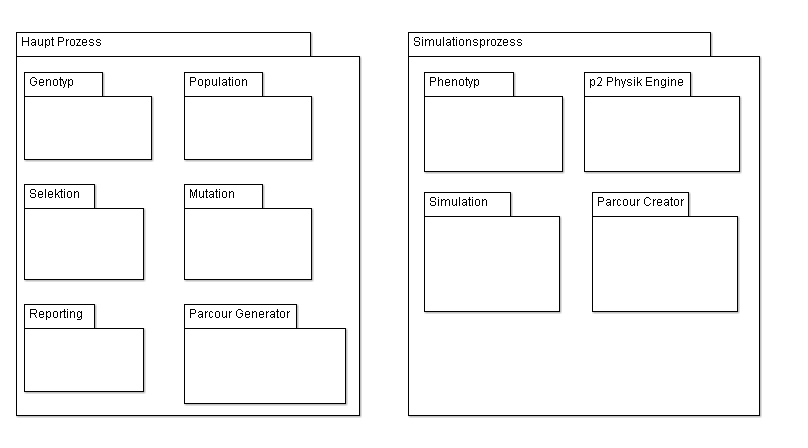
\includegraphics[scale=0.45,center]{graphics/haupt_simulations_prozess}
      \caption{Haupt- und Simulationsprozess\label{fig:hauptSimuProzesse}}
    \end{figure}
    \begin{figure}[H]
      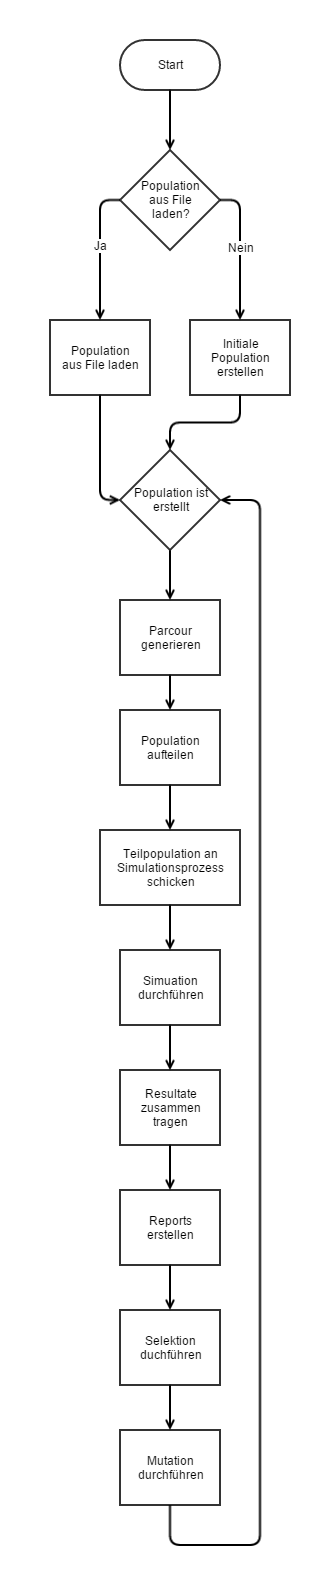
\includegraphics[scale=0.45,center]{graphics/ablauf}
      \caption{Ablauf der Simulation\label{fig:ablauf}}
    \end{figure}

    \subsection{Initiale Population\label{sec:initPop}}

      Als erster Schritt muss eine initiale Population erstellt werden. Die Populationsgrösse kann frei gewählt werden.
      Pro Simulationsprozess können etwa 15 Individuen flüssig berechnet werden.
      Dies bedeutet das die optimale Populationsgrösse  \( Anzahl(CPU Kerne) * 15 \) beträgt.
      Dieser Wert wurde durch mehrere Versuche mit unterschiedlichen Prozessoren gefunden.
      Es werden jeweils Individuen mit 4, 5, 6, 7 und 8 Körperpunkten~(\vref{sub:DesignBody}) zufällig generiert.
      Die Verantwortliche Klasse in Javascript ist der InitialPopulationGenerator.
      Das Endprodukt dieses Schrittes ist eine Population bestehenden aus den Genotypen der Individuen.

    \subsection{Parcours-Generierung\label{sec:Parcour Generierung}}

      Der Parcours wird zufällig generiert. Am Anfang wird ein einfacher und flacher Parcours generiert.
      Mit zunehmenden Iterationen steigt die Schwierigkeit des Parcours,
      das heisst es werden höhere Steigungen und Punkte mit höheren Y-Koordinaten vorkommen.
      \vref{fig:parcours1},~\vref{fig:parcours2} und~\vref{fig:parcours3} zeigen
      wie der Parcours mit zunehmenden Generationen schwieriger wird.
      Der ParcourGenerator ist die Verantwortliche Klasse in Javascript,
      welche mit Hilfe von Obergrenzen von Werten einen Parcours generieren kann.
      Wie unter~\ref{sec:Konfiguration} erwähnt,
      wird je nach Einstellung der Parcours nach jeder Generation neu generiert (allgemeine Lösung) oder
      er wird wiederverwendet (evolvieren auf Evolvierbarkeit).
      Der Parcours wird im ParcourGenerator generiert (Hauptprozess) und
      von den jeweiligen Simulationsprozessen mit Hilfe vom ParcourCreator in der \gls{PhysicsEngine} erstellt.

      \vspace{1cm}

      \begin{figure}[H]
        \centering
        %
% Concept parcours
%

% !TEX root = ../main.tex


\begin{tikzpicture}[scale=\textwidth/20cm]

  \coordinate (P0) at (0,0);
  \coordinate (P1) at (0,0.5);
  \coordinate (P2) at (20,0.5);
  \coordinate (P3) at (20,0);

  % Draw parcours
  \draw [fill=black] (P0) -- (P1) -- (P2) -- (P3) -- cycle;

\end{tikzpicture}

        \caption{flacher Start-Parcours 1. Generation\label{fig:parcours1}}
      \end{figure}

      \begin{figure}[H]
        \centering
        %
% Concept parcours
%

% !TEX root = ../main.tex


\begin{tikzpicture}[scale=\textwidth/20cm]

  \coordinate (P0) at (0,0);
  \coordinate (P00) at (0,0.5);
  \coordinate (P1) at (2,0.5);
  \coordinate (P2) at (5,0.8);
  \coordinate (P3) at (8,0.8);
  \coordinate (P4) at (12,0.5);
  \coordinate (P5) at (14,0.5);
  \coordinate (P6) at (16,0.65);
  \coordinate (P7) at (17,0.65);
  \coordinate (P8) at (19,0.8);
  \coordinate (P9) at (20,1);
  \coordinate (P10) at (20,0);

  % Draw parcours
  \draw [fill=black] (P0) -- (P00) -- (P1) -- (P2) -- (P3) -- (P4) -- (P5) -- (P6) -- (P7) -- (P8) -- (P9) -- (P10) -- cycle;

\end{tikzpicture}

        \caption{Parcours 100. Generation\label{fig:parcours2}}
      \end{figure}

      \begin{figure}[H]
        \centering
        %
% Concept parcours
%

% !TEX root = ../main.tex


\begin{tikzpicture}[scale=\textwidth/20cm]

  \coordinate (P0) at (0,0);
  \coordinate (P00) at (0,0.5);
  \coordinate (P1) at (2,0.5);
  \coordinate (P2) at (5,1.5);
  \coordinate (P3) at (8,2);
  \coordinate (P4) at (12,1.3);
  \coordinate (P5) at (14,1.3);
  \coordinate (P6) at (16,0.65);
  \coordinate (P7) at (17,0.5);
  \coordinate (P8) at (19,0.8);
  \coordinate (P9) at (20,1);
  \coordinate (P10) at (20,0);

  % Draw parcours
  \draw [fill=black] (P0) -- (P00) -- (P1) -- (P2) -- (P3) -- (P4) -- (P5) -- (P6) -- (P7) -- (P8) -- (P9) -- (P10) -- cycle;

\end{tikzpicture}

        \caption{Parcours 1000. Generation\label{fig:parcours3}}
      \end{figure}

      \subsection{Simulation\label{sec:simulation}}

        Nachdem eine neue Population und ein neuer Parcours erstellt worden ist.
        Muss eine Simulation durchgeführt werden um den Fitnesswert der Individuen zu bestimmen.
        Die Verantwortliche Klasse ist die SimulationWorld.
        Zuerst muss jeder Genotyp zu einem Phänotyp abgebildet werden.
        Anschliessend muss der Parcours aus dem Blueprint erstellt werden. % TODO referenz?
        Erst dann kann mit der Simulation begonnen werden.
        Die SimulationWorld merkt sich zu jedem Individuum die Position.
        Individuen welche sich während 4 Sekunden kaum bewegt haben,
        werden aus der laufenden Simulation entfernt und ihr Fitnesswert wird abgespeichert.
        Die Simulation kann wie unter~\ref{sec:Konfiguration} schon erwähnt, parallelisiert werden. \\
        Es wird dann jeweils für \( Populationsgrösse / Anzahl Simulationsprozesse \) Individuen eine eigene Simulation erstellt.

    \subsection{Reporting\label{subsec:Reporting}}

      Das Reporting-Modul hilft nach einer Simulation alle wichtigen Daten festzuhalten.
      Mithilfe einer Funktion welche eine Population als Parameter entgegennimmt,
      werden die Reports erstellt.
      Es existieren folgende Typen von Reports:

      \begin{itemize}

        \item Fitness Graph Average Report: Enthält Koordinaten,
          um einen Graphen über die durchschnittliche Fitness pro Generation zu erstellen.

        \item Fitness Graph Best Report: Enthält Koordinaten,
          um einen Graphen über das beste Individuum der Generation zu erstellen.

        \item Genotype Blue Print Report: Enthält pro Generation ein \gls{JSON}-Objekt,
          das Informationen über die ganze Population enthält.

        \item Fitness Graph Average Report bp x: Für diesen Typ von Report gibt es jeweils einen für alle Individuen mit Body Points Anzahl x.
              Ansonsten gleich wie der Fitness Graph Average Report.

        \item Diversity Report: Enthält die Berechnung der Punktstreuung für eine Generation.
          Die Punktstreuung berechnet sich wie folgt:

        \begin{itemize}
          \item Erstellen von Vektoren der Genome. Jede Eigenschaft des Genoms wird in einen numerischen Wert konvertiert. \( V_d \)
          \item Alle Vektoren werden summiert. Die Summe wird als \(V_s\) bezeichnet.
          \item Der Schwerpunktvektor wird gebildet: \( V_s / Anzahl(V_d) = V_{schwer} \)
          \item Von jedem \(V_d\) wird \(V_{schwer}\) subtrahiert  \( V_d - V_{schwer}  = V_{d2} \)
          \item Nun werden alle \(V_{d2}\) normiert, quadriert \( norm{(V_{d2})}^2 = d \)
          \item Abschliessend werden alle \(d\) zusammengezählt und durch \(Anzahl(V_d)\) dividiert. So wird ein Mass für die Punktestreuung gewonnen.
        \end{itemize}
      \end{itemize}

    \subsection{Selektion\label{sec:Selektion}}

      \citet[S.33]{book:bioInspired} schreiben,
      dass Turnierbasierte-Selektion oft bei evolutionärer Programmierung eingesetzt wird.
      Turnierbasierte-Selektion hat den Vorteil, dass die Diversität erhalten bleibt,
      bei gleichzeitig guter Selektion der fittesten Individuen.
      Aufgrund der Empfehlung von D. Floreano und C. Mattiussi und der Erhaltung der Diversität,
      wurde entschieden Turnierbasierte-Selektion einzusetzen.

    \subsection{Mutation\label{sec:Mutation}}

      Auf die Selektionsstrategie folgt nun die Mutation der Individuen.
      Bei der Mutation wird über jede Eigenschaft des Individuums iteriert und
      diese wird mit einer bestimmten Wahrscheinlichkeit (PROBABILITY) und um einen bestimmten Wert (STEP) verändert.
      PROBABILITY kann Werte zwischen 0 und 1 annehmen, STEP hat keine Einschränkungen.
      Nachdem für jedes Attribut diese Werte definiert worden sind, kann die Mutation stattfinden.
      Limiten~(\vref{sub:IntroReqLimit}) wurden definiert, um nicht gewinnbringende Lösung zu verhindern.
      Die Position eines Beins wird unter einer zusätzlichen Bedingung mutiert. Falls sich der Körper so verändert hat,
      dass ein Bein ausserhalb des Körpers ist, wird die Position zufällig neu bestimmt.
      Die Mutation läuft wie die Simulation parallel ab, das heisst, sie kann von mehreren CPU-Kernen profitieren.

      \subsubsection{Hypothese zur Mutation\label{subsub:hypoMut}}

        Es wird die Hypothese aufgestellt,
        dass kleinere Mutationswahrscheinlichkeiten bessere Fitnesswerte liefern als grosse.
        Die Annahme besteht darin, dass die Evolution der Individuen gebremst wird,
        falls grosse Mutationswahrscheinlichkeiten eingesetzt werden.

    \subsection{Abbruchkriterium}

      Der evolutionäre Algorithmus wird solange ausgeführt, bis der Anwender sich entscheidet ihn abzubrechen.
      Theoretisch wäre möglich abzubrechen, wenn ein bestimmter Fitnesswert erreicht wird.
      Ohne automatischen Abbruch ist mehr Flexibilität gewährleistet,
      der Anwender kann die Reports immer wieder überprüfen und entscheiden,
      ob die Individuen den Ansprüchen genügen.

    \subsection{Domänenmodell\label{sub:domMod}}

      Das Domänenmodell beschreibt den Zusammenhang der verschiedenen Klassen und Objekten.
      \vref{fig:mainProcess} beschreibt den Haupt- und~\vref{fig:simulationProcess} den Simulationsprozess.
      \begin{figure}[H]
        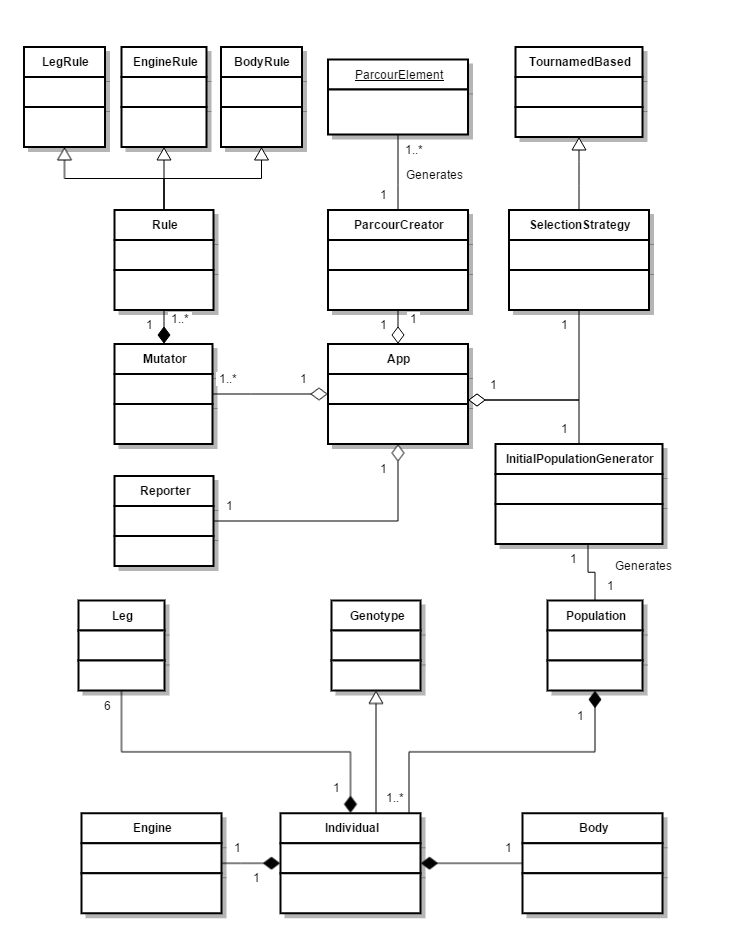
\includegraphics[scale=0.6,center]{graphics/main_process}
        \caption{Domänenmodell, Hauptprozess\label{fig:mainProcess}}
      \end{figure}
      \begin{figure}[H]
        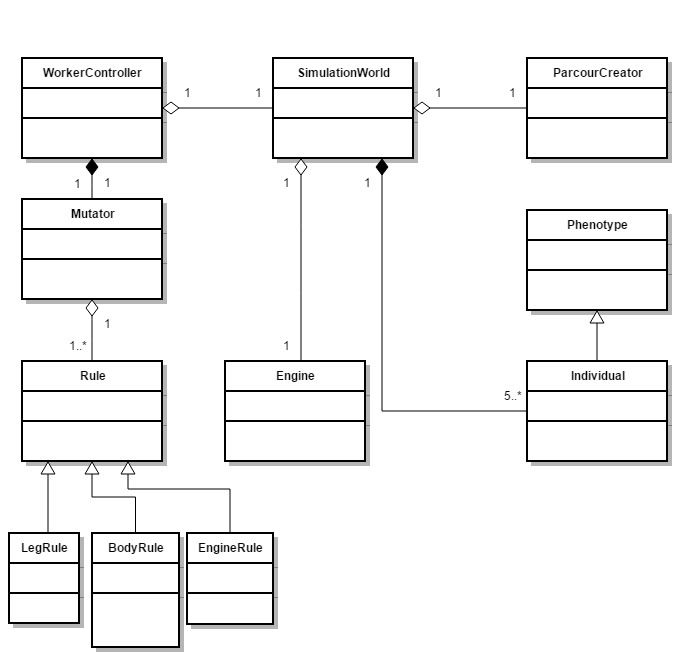
\includegraphics[scale=0.6,center]{graphics/simulation_process}
        \caption{Domänenmodell, Simulationsprozess\label{fig:simulationProcess}}
      \end{figure}
